\section{From $\Gbox$ to $\Ginf$ (Proving Proposition \ref{prop:convergence_average_clustering_P_n})}\label{sec:clustering_Pn_to_P}

In this section we shall relate the clustering in the finite box model $\Gbox$ to that of the infinite model. The main goal is to prove Proposition~\ref{prop:convergence_average_clustering_P_n} which states that
\[
	\left|\Exp{c^\ast(k_n; \Gbox)} - \gamma(k_n)\right| = \smallO{s(k_n)}.
\] 

Recall that $\Gbox$ is obtained by restricting the Poisson point process $\PPP$ to the box $\Rcal = (-I_n, I_n] \times (0, R_n]$, with $I_n = \frac{\pi}{2} e^{R_n/2}$ and connecting two points $p_1, p_2 \in \Rcal$ if and only if $|x_1 - x_2|_{\pi e^{R_n/2}} \le e^{(y_1 + y_2)/2}$. We also recall that by definition of the norm $|.|_{\pi e^{R_n/2}}$ the left and right boundaries of $\Rcal$ are identified. See Section~\ref{ssec:finite_model} for more details. Due to this identification of the boundaries some triples of nodes that form a triangle in the finite box model do not form a triangle in the infinite model. Therefore, to establish the required result we need to compute the asymptotic difference between triangle counts in both models.


%\TM{ This last bit of the sentence is already contained in the fact we us $|.|_{\pi e^{R_n/2}}$. To me it does not add anything, except possibly confusion. } \PvdH{I have updated this and just added a reminder of this.}

%In this section we shall compute the asymptotic difference between triangle counts in the finite box and infinite model. First we recall the definition of $\Kcal_{C}(k_n)$
%\[
%	\Kcal_C(k_n) = \left\{y \in \R_+ : \frac{k_n - C \sqrt{k_n \log(k_n)}}{\xi} \le e^{\frac{y}{2}}
%	\le \frac{k_n + C \sqrt{k_n \log(k_n)}}{\xi} \right\},	
%\]
%\TM{ Typo : $p\in\R$. Do you mean $\Rcal$? Or maybe 
%$\R \times \R^+$? Still not sure that max and min in defn add anything. } \PvdH{It was a typo and is corrected. I have removed the max and min.}
%with
%\[
%	\kappa_n := \begin{cases}
%		\log(n) &\mbox{if } k_n = \bigT{1},\\
%		\sqrt{k_n \log(k_n)} &\mbox{else.}
%	\end{cases}
%\]
%\TM{ Same issue as before. }
%In addition we note that the function $\phi_n(y)$ in Lemma~\ref{lem:average_degree_P_n} satisfies
%\[
%	\phi_n(y) = \bigT{e^{-(\alpha - \frac{1}{2})(R_n - y)}},
%\]
%as $R_n - y \to \infty$. Since $e^{y/2} = \bigT{k_n} = \smallO{e^{R_n}}$ as $n \to \infty$, uniformly on $\Kcal_C(k_n)$, it follows that $\phi_n(y) = \bigT{k_n^{2\alpha - 1} n^{-(2\alpha - 1)}}$, uniformly on $\Kcal_C$. This yields the following useful corollary to Lemma~\ref{lem:average_degree_P_n}.
%
%\begin{corollary}\label{cor:average_degree_P_n_K}
%Let $\alpha > \frac{1}{2}$, $C > 0$. Then, for all $y \in \Kcal_{C}(k_n)$,
%\[
%	\mu(\BallPon{y}) = \mu(\BallPo{y})\left(1 - \bigT{k_n^{2\alpha - 1} n^{-(2\alpha - 1)}}\right).
%\]
%\TM{ I don't follow. Spell it out. }\PvdH{I added additional explanation above. Please see if this solves the confusion.}
%
%\end{corollary}




%We now turn to the task of calculating the expected number of triangles of a node at height $y$, for both the infinite model and the finite box model. 
For any $p \in \R \times \R_+$ we define for the finite box model,
\[
	T_{\text{box}}(p) = \sum^{\ne}_{p_1, p_2 \in \Pcal \setminus \{p\}} T_{\text{box}}(p,p_1,p_2)
\]
where the sum is over all distinct pairs in $\Pcal \setminus p$ and
\[
	T_{\text{box}}(p,p_1,p_2) = \ind{p_1 \in \BallPon{p}}\ind{p_2 \in \BallPon{p}}\ind{p_2 \in \BallPon{p_1}}.
\]
Similarly, for the infinite model we define
\[
	T_\infty(y) = \sum_{p_1, p_2 \in \Pcal \setminus (0,y)}^{\ne} T_\infty(y,p_1,p_2),
\]
where
\[
	T_{\infty}(y,p_1,p_2) = \ind{p_1 \in \BallPo{y}}\ind{p_2 \in \BallPo{y}}\ind{p_2 \in \BallPo{p_1}}.
\]
Here we slightly abuse notation and write $\BallPo{y}$ for $\BallPo{(0,y)}$. We will adopt this notational convention throughout the remainder of this section, to keep notation concise.

We will first relate $\gamma(k_n)$ and $\Exp{c^\ast(k_n; \Gbox)}$ using $T_\infty(y)$ and $T_{\text{box}}(y)$. Recall the definition of $\Kcal_{C}(k_n)$
\[
	\Kcal_C(k_n) = \left\{y \in \R_+ : \frac{k_n - C \sqrt{k_n \log(k_n)}}{\xi} \le e^{\frac{y}{2}}
	\le \frac{k_n + C \sqrt{k_n \log(k_n)}}{\xi} \right\},	
\]

\begin{lemma}
Let $\gamma(k_n)$ be defined as in~\eqref{eq:gammakint}. Then as $n \to \infty$
\begin{equation}\label{eq:alt_gamma_kn}
	\gamma(k_n) = (1+\smallO{1})\frac{1}{k_n^2 p_{k_n}} \int_{\Kcal_{C}(k_n)} \Exp{T_\infty(y)} \rho(y,k) 
				\alpha e^{-\alpha y} \dd y. 
\end{equation}
Moreover,
\begin{equation}\label{eq:alt_c_ast_kn}
	\Exp{c^\ast(k_n;\Gbox)} = (1 + \smallO{1}) \frac{1}{k_n^2 p_{k_n}} \int_{\Kcal_{C}(k_n)} \Exp{T_{\text{box}}(y)}
		\rho(y,k_n) \alpha e^{-\alpha y} \dd y
\end{equation}
as $n \to \infty$,
\end{lemma}

\begin{proof}
Recall that 
\[
	P(y) = \Exp{\ind{u_1 \in \BallPo{u_2}}},
\]
where $u_1$ and $u_2$ are independent and distributed according to the probability density \\$\Mu{\BallPo{y}}^{-1} \ind{u_i \in \BallPo{y}} f(x_i, y_i)$. It then follows from the Campbell-Mecke formula that
\begin{align*}
	\Exp{T_\infty(y)} &= \int \ind{p_1 \in \BallPo{y}}\ind{p_2 \in \BallPo{y}}
		\ind{p_2 \in \BallPo{p_1}} f(x_1,y_1) f(x_2,y_2) \dd x_1 \dd x_2 \dd y_1 \dd y_2\\
	&= \Mu{\BallPo{y}}^2 P(y).
\end{align*}
It then follows that,
\begin{align*}
	\gamma(k_n) &= \frac{1}{p_{k_n}} \cdot \int_0^\infty P(y) \rho(y,k) \alpha e^{-\alpha y} \dd y \\
	&= \frac{1}{p_{k_n}} \int_0^\infty \Exp{T_\infty(y)} \Mu{\BallPo{y}}^{-2} \rho(y,k) 
		\alpha e^{-\alpha y_0} \dd y_0\\
	&= (1+ \smallO{1}) \frac{1}{k_n^2 p_{k_n}} \int_0^\infty \Exp{T_\infty(y)} \rho(y,k) \alpha e^{-\alpha y} \dd y_0,
\end{align*}
where the last line is due to a concentration of heights argument.

For~\eqref{eq:alt_c_ast_kn} we recall that
\[
	c^\ast(k_n; \Gbox) = \frac{1}{\Exp{\Nbox(k_n)}} \sum_{p \in \Pcal} c_{\text{box}}(p)\ind{\Dbox(p) = k_n},
\]
where $c_{\text{box}}(p)$ can be expressed as
\[
	c_{\text{box}}(p) = \frac{1}{\binom{\Dbox(p)}{2}} \sum_{p_1, p_2 \in \Pcal \setminus p}^{\ne} T_{\text{box}}(p,p_1,p_2)
	= \frac{T_{\text{box}}(p)}{\binom{\Dbox(p)}{2}}.
\]
By the Campbell-Mecje formula
\begin{align*}
	\Exp{c^\ast(k_n; \Gbox)} 
	&= \frac{1}{\Exp{\Nbox(k_n)}} \int_{\Rcal} \Exp{c_{\text{box}}(p)\ind{\Dbox(p) = k_n}} f(x,y) \dd x \dd y\\
	&= \frac{1}{\Exp{\Nbox(k_n)}} \int_{\Rcal} \CExp{c_{\text{box}}(p)}{\Dbox(p) = k_n}\rho_{\text{box}}(p,k_n) 
		f(x,y) \dd x \dd y\\
	&= (1+\smallO{1})\frac{n}{\Exp{\Nbox(k_n)}} \int_{\Kcal_C(k_n)} \CExp{c_{\text{box}}(y)}{\Dbox(y) = k_n}
		\rho(y,k_n) \alpha e^{-\alpha y} \dd y,
\end{align*}
where the last line follows from a concentration of heights argument, for which we used that $\CExp{c_{\text{box}}(y)}{\Dbox(y) = k_n} \le 1$. To analyze the conditional expectation we observe that, similar to the analysis of $\gamma(k_n)$, conditioned on there being $k_n$ points in $\BallPon{y}$, each point $u_i = (x_i,y_i)$ is independently distributed according to the probability density $\Mu{\BallPon{y}}^{-1} \ind{u_i \in \BallPon{y}} f(x_i,y_i)$. Therefore,
\begin{align*}
	\CExp{c_{\text{box}}(y)}{\Dbox(y) = k_n}
	&= \binom{k_n}{2}^{-1} \Exp{\sum_{1 \le i < j \le k_n} \ind{u_i \in \BallPon{u_j}}} \\
	&= \Exp{u_1 \in \BallPon{u_2}} \\
	&= \Mu{\BallPon{y}}^{-2} \iint T_{\text{box}}(y,p_1,p_2) f(x_1,y_1) f(x_2,y_2) 
		\dd x_1 \dd y_1 \dd x_2 \dd y_2\\
	&= \Mu{\BallPon{y}}^{-2} \Exp{T_{\text{box}}(y)}.
\end{align*}
and thus, by applying a concentration of heights argument on $\Mu{\BallPon{y}}^{-2}$,
\[
	\Exp{c^\ast(k_n; \Gbox)} = (1 + \smallO{1}) \frac{n \Mu{\BallPon{2\log(k_n/\xi)}}^{-2}}{\Exp{\Nbox(k_n)}} \int_{\Kcal_C(k_n)} \Exp{T_{\text{box}}(y)} \rho(y,k_n) \alpha e^{-\alpha y} \dd y.
\]
To finish the argument, we first note that $\Mu{\BallPon{2\log(k_n/\xi)}}^{-2} = (1+\smallO{1})k_n^2$, while
\[
	\Exp{N_{\text{box}}(k_n)} = \int_{\Rcal} \rho_{\text{box}}(y,k_n) f(x,y) \dd x \dd y,
\]
so that by a concentration of heights argument,
\[
	\Exp{N_{\text{box}}(k_n)} = (1+o(1)) n \int_{0}^\infty \rho(y,k_n) \alpha e^{-\alpha y} \dd y 
	= (1+\smallO{1}) n p_{k_n}.
\]
We therefore conclude that
\[
	\Exp{c^\ast(k_n; \Gbox)} = (1 + \smallO{1}) \frac{1}{k_n^2 p_{k_n}} \int_{\Kcal_C(k_n)} 
		\Exp{T_{\text{box}}(y)} \rho(y,k_n) \alpha e^{-\alpha y} \dd y.
\]


%Next recall the definition of $\Kcal_{C}(k_n)$, see~\eqref{eq:def_K_C_set}, and note that for all $y_0 \in \Kcal_{C}(k_n)$, $\mu(y) = (1+\smallO{1})k_n$. Then Lemma~\ref{lem:concentration_argument} implies that, as $n \to \infty$,
%\begin{align*}
%	&\hspace{-30pt} \int_0^\infty \Exp{T_\infty(y_0)} \left(\frac{\mu(y)^2}{2}\right)^{-1} \rho(y_0,k) 
%		\alpha e^{-\alpha y_0} \dd y_0\\
%	&= (1+ \smallO{1}) \binom{k_n}{2}^{-1} \int_0^\infty \Exp{T_\infty(y_0)} \rho(y_0,k) \alpha e^{-\alpha y_0} \dd y_0,
%\end{align*}
%which finishes the proof.
\end{proof}


%
%
%For the finite box model we have, by the Campbell-Mecke formula,
%\begin{align*}
%	\Exp{c^\ast(k_n, \Gbox)}
%	&= \frac{1}{\binom{k_n}{2}\Exp{\Nbox(k_n)}} \int_{\Rcal} \Exp{T_{\text{box}}(p) \ind{\text{deg}(p) = k_n}} f(x,y) 
%		\dd x \dd y\\
%	&= \frac{n}{\binom{k_n}{2}N_{\Gbox}(k_n)} \int_0^{R} \CExp{T_{\text{box}}(y_0)}{\text{deg}(y_0) = k_n} 
%		\rho_{\text{box}}(y,k_n) \alpha e^{-\alpha y_0} \dd y_0,
%\end{align*}
%where the last line follows since the Poisson point process is invariant in $x$ and by slightly abusing notation $T_{\text{box}}(y_0) = T_{\text{box}}(0,y_0)$. Next we note that 
%\[
%	\Exp{N_{\text{box}}(k_n)} = \int_{\Rcal} \rho_{\text{box}}(y,k_n) f(x,y) \dd x \dd y,
%\]
%so that by a concentration of heights argument, see Corollary~\ref{cor:concentration_heights_asymptotics_n},
%\[
%	\Exp{N_{\text{box}}(k_n)} = (1+o(1)) \alpha n \int_{0}^\infty \rho(y,k_n) e^{-\alpha y} \dd y 
%	= (1+\smallO{1}) n p_{k_n}.
%\]
%Since $\Exp{T_{\text{box}}(y_0)\ind{\text{deg}(y_0) = k_n}} \le \binom{k_n}{2}$, and Another concentration of heights argument yields
%\[
%	\int_0^{R} \Exp{T_{\text{box}}(y_0)} \rho_{\text{box}}(y_0,k_n) \alpha e^{-\alpha y_0} \dd y_0
%	= (1 + \smallO{1}) \int_{\Kcal_{C}(k_n)} \Exp{T_{\text{box}}(y_0)} \rho(y_0,k_n) \alpha e^{-\alpha y_0} \dd y_0
%\]
%and hence
%\begin{equation}\label{eq:approx_c_ast_Gbox}
%	c^\ast(k_n, \Gbox)  = (1 + \smallO{1})\frac{1}{p_{k_n}} \int_{\Kcal_{C}(k_n)} \binom{k_n}{2}^{-1} \Exp{T_{\text{box}}(y_0)} \rho(y_0,k_n) \alpha e^{-\alpha y_0} \dd y_0.
%\end{equation}

Comparing~\eqref{eq:alt_gamma_kn} and~\eqref{eq:alt_c_ast_kn}, we conclude that to prove Proposition~\ref{prop:convergence_average_clustering_P_n} it is enough to show that
\begin{equation}\label{eq:triangle_diff_main_term}
	 \left|\int_{\Kcal_{C}(k_n)} \Exp{T_{\text{box}}(y) - T_\infty(y)}
	\rho(y,k) \alpha e^{-\alpha y} \, d y \right|
	= \smallO{s(k_n)p_{k_n}k_n^2},
\end{equation}
which means we have to compute the expected difference in triangles between both models.


%it follows that
%\[
%	\Exp{T_{\text{box}}(p_0)} = \frac{1}{2}\iint_{\Rcal^2} T_{\text{box}}(p_0,p_1,p_2)
%	f(x_1,y_1) f(x_1,y_1) \, dx_1 \, dx_2 \, dy_1 \, dy_2,
%\]
%
%\TM{ $p$ is supposed to be $p_0$ I assume. }\PvdH{Indeed. It has been corrected.}

\subsection{Comparing triangles between $\Ginf$ and $\Gbox$}

To analyze $T_{\text{box}}(y_0) - T_\infty(y_0)$ we first reiterate that the difference between the indicator $\ind{p_1 \in \BallPon{p}}$ in the finite box model and $\ind{p_1 \in \BallPo{p}}$ is that in $\Gbox$ we identified the boundaries of the interval $[-\frac{\pi}{2}e^{R_n/2}, \frac{\pi}{2} e^{R_n/2}]$ and we stop at height $y = R_n$. This induces a difference in triangle counts between both models. 
To see this, note that for any $p = (x,y)$ with $0 \le y \le R_n$ we have that $\BallPon{p} = \BallPo{p} \cap \Rcal$. This means that if $p^\prime, p_2 \in \BallPon{p}$ and $p_2 \in \BallPo{p^\prime} \cap \Rcal$ then $p_2 \in \BallPon{p} \cap \BallPon{p^\prime}$ and hence $(p,p^\prime,p_2)$ form a triangle both in $\Gbox$ and $\Ginf$. However, it could happen that there are points in the intersection $\BallPon{p} \cap \BallPon{p^\prime}$ that are not in $\BallPo{p} \cap \BallPo{p^\prime}$. Let us denote this region by $\mathcal{T}(p,p^\prime)$, see Figure~\ref{fig:comparing_triangles_diff_intersections} for an example of this region. Then, any $p_2 \in \mathcal{T}(p,p^\prime)$ creates a triangle with $p$ and $p^\prime$ in $\Gbox$ that is not present in $\Ginf$. Finally, any point $p_2 \in \BallPo{p} \cap \BallPo{p^\prime}$ with height $y_2 > R$ creates a triangle with $p, p^\prime$ in $\Ginf$ but not in $\Gbox$.

Let us now define the following triangle count function
\[
	\widetilde{T}_{\text{box}}(p_0) = \sum_{(p_1, p_2) \in \Pcal \setminus \{p_0\}}^{\ne} 
		\widetilde{T}_{\text{box}}(p_0,p_1,p_2).
\]
where
\[
	\widetilde{T}_{\text{box}}(p_0,p_1,p_2) = \ind{p_1 \in \BallPon{p}}\ind{p_2 \in \BallPon{p}}\ind{p_2 \in \BallPo{p_1} \cap \Rcal}.
\]
Then $\widetilde{T}_{\text{box}}(p_0)$ only counts those triangles attached to $p_0$ that exist in both $\Gbox$ and $\Ginf$ and thus, by definition of the region $\mathcal{T}(p_0,p_1)$,
\[
	T_{\text{box}}(p_0) - \widetilde{T}_{\text{box}}(p_0)
	= \sum_{p_1, p_2 \in \Pcal \setminus \{p_0\}}^{\ne} \ind{p_1 \in \BallPon{p_0}} 
			\ind{p_2 \in \mathcal{T}(p_0, p_1)}.
\]
%Thus, $\widetilde{T}_{\text{box}}(p_0)$ only count those triangles $(p_0,p_1,p_2)$ that also exist in $\Ginf$.
%Observe that the difference between $\widetilde{T}_{\text{box}}(p_0)$ and $T_{\text{box}}(p_0)$ is in the last indicator in $\widetilde{T}_{\text{box}}(p_0,p_1,p_2)$.  counts those points $p_2$ in the box $\Rcal$ that are in the neighbourhood $\BallPo{p_1}$ of $p_1$ in the infinite model. Thus, $\widetilde{T}_{\text{box}}(p_0)$ only count those triangles $(p_0,p_1,p_2)$ that also exist in $\Ginf$.

  

The next result, which is crucial for the proof of Proposition~\ref{prop:convergence_average_clustering_P_n}, computes the expected measure of $\mathcal{T}(p,p^\prime)$ with respect to $p^\prime$. 

\begin{lemma}\label{lem:clustering_error_T_term}
Let $p_0 = (0,y)$ with $y \in \Kcal_{C}(k_n)$. Then as $n \to \infty$,
\[
	\Exp{\left|T_{\text{box}}(p_0) - \widetilde{T}_{\text{box}}(p_0)\right|}
	= y \, \bigO{n^{-(2\alpha - 1)}} + e^{y}\,\bigO{n^{-(4\alpha-2)}}.
\]
%\[
%	\int_{\Rcal} \mu\left(\mathcal{T}(p,p^\prime)(p_0,p_1)\right) f(x_1,y_1) 
%	\dd x_1 \dd y_1 = \bigO{y n^{-(2\alpha - 1)} + n^{-(2\alpha-1)} e^{y}}
%\]
\end{lemma}

The proof of the lemma is not difficult but cumbersome, since it involves computing many different integrals. We postpone this proof till the end of this section and proceed with the main goal, proving Proposition~\ref{prop:convergence_average_clustering_P_n}. 

First we state a small lemma about the scaling of $s(k_n)$ that will be very useful.  

\begin{lemma}\label{lem:scaling_s_alpha}
Let $s(k_n)$ be as defined in \eqref{eq:def_scaling_function}. Then for any $k_n = \smallO{n^{\frac{1}{2\alpha + 1}}}$, as $n \to \infty$,
\[
	n^{-(2\alpha - 1)} = \smallO{s(k_n)}.
\]
\end{lemma}

\begin{proof}
First let $\frac{1}{2} < \alpha < \frac{3}{4}$. Then
\[
	n^{-(2\alpha - 1)}s(k_n)^{-1} = n^{-(2\alpha -1)}k_n^{4\alpha - 2}
	= \smallO{n^{-(2\alpha - 1) + \frac{4\alpha - 2}{2\alpha + 1}}} 
	= \smallO{n^{-\frac{4\alpha^2 - 4\alpha + 1}{2\alpha + 1}}}
	= \smallO{1},
\]
since $4\alpha^2 - 4\alpha + 1 > 0$ for all $\alpha > \frac{1}{2}$. Similarly, for $\alpha \ge \frac{3}{4}$ we have
that $4\alpha^2 > 2$ and hence,
\[
	n^{-(2\alpha - 1)} s_{\alpha}(k_n) = \smallO{n^{-(2\alpha - 1)} k_n} = \smallO{n^{-\frac{4\alpha^2 - 2}{2\alpha + 1}}}
	= \smallO{1}.
\]
\end{proof}

We now proceed with proving the main result of this section.

\begin{proof}[Proof of Proposition~\ref{prop:convergence_average_clustering_P_n}]
Let us write $\Rcal^\prime := (\R \times \R_+) \setminus \Rcal$ and let $p_0 = (0,y)$ denote the typical point. Next we recall that it is enough to show~\eqref{eq:triangle_diff_main_term}, so that in particular we have that $y \in \Kcal_{C}(k_n)$.

Now
\begin{align*}
	\left|T_{\text{box}}(p_0) - T_{\infty}(p_0)\right| 
	&= \left|T_{\text{box}}(p_0) - \widetilde{T}_{\text{box}}(p_0)\right| 
		+ \sum_{p_1, p_2 \in \Pcal \cap \Rcal^\prime}^{\ne} T_{\infty}(p_0,p_1,p_2),
\end{align*}
so that by the Campbell-Mecke formula
\begin{align*}
	\left|\Exp{T_{\text{box}}(p_0) - T_{\infty}(p_0)}\right|
	&\le \Exp{\left|T_{\text{box}}(p_0) - \widetilde{T}_{\text{box}}(p_0)\right|}\\
	&\hspace{10pt}+ \int_{\Rcal^\prime}\int_{\Rcal^\prime} T_{\infty}(p_0,p_1,p_2) f(x_1,y_1) f(x_2,y_2)
		\dd x_2 \dd y_2 \dd x_1 \dd y_1. 
\end{align*}

\TM{ in the 1st integral we could have restricted to the ball of $p$, and possibly saved a lot. Does that not help? }\PvdH{the first integral is taken care of by another Lemma so it does not matter I think.}
The first part is taken care of by Lemma~\ref{lem:clustering_error_T_term}. For the other integral we have
\begin{align*}
	&\hspace{-30pt}\iint_{\Rcal^\prime} T_{\infty}(p_0,p_1,p_2) f(x_1,y_1) f(x_2,y_2)
		\dd x_2 \dd y_2 \dd x_1 \dd y_1\\
	&\le \left(\int_{\Rcal^\prime} \ind{p_1 \in \BallPo{p_0}} f(x_1,y_1) \dd x_1 \dd y_1\right)^2
		= \bigO{\left(e^{y/2} \int_{R_n}^\infty e^{-(\alpha - \frac{1}{2})y_1} \dd y_1\right)^2}\\
	&= \bigO{e^{y} e^{-(2\alpha-1)R_n}} = \bigO{e^y n^{-(4\alpha - 2)}}.
\end{align*}
%\TM{ Typo : $f_{\mu, \nu}$? Also give more details how line 3 follows. }
Thus we conclude, using Lemma~\ref{lem:clustering_error_T_term}, that,
\begin{equation}\label{eq:triangle_count_diff_scaling}
	\left|\Exp{T_{\text{box}}(p_0) - T_{\infty}(p_0)}\right| = \bigO{y n^{-(2\alpha - 1)} + n^{-(4\alpha-2)} e^{y}}.
\end{equation}
Therefore, on $\Kcal_C(k_n)$, 
\begin{align*}
	&\hspace{-30pt}\int_{\Kcal_{C}(k_n)} \rho(y_0,k_n) \left|\Exp{T_{\text{box}}(p_0) - T_{\infty}(p_0)}\right| 
		e^{-\alpha y_0} \dd y_0\\
	&= \bigO{1} \left(\log(k_n) n^{-(2\alpha - 1)} + k_n^2 n^{-(4\alpha - 2)} \right) 
		\int_{0}^\infty \rho(y_0,k_n) e^{-\alpha y_0} \dd y_0\\
	&= \bigO{1} \left(\log(k_n) n^{-(2\alpha - 1)} + k_n^2 n^{-(4\alpha - 2)} \right) p_{k_n} = \smallO{s(k_n) p_{k_n} k_n^2},
\end{align*}
%\TM{ Typo : $e^{-\alpha}$ }
where the last part follows from Lemma~\ref{lem:scaling_s_alpha} and the fact that $s(k_n)^2 = \smallO{s(k_n)}$. This establishes~\eqref{eq:triangle_diff_main_term} and hence finishes the proof.
%
% \TM{ Also justify penultimate step! }\PvdH{What do you mean?}
%To finish the argument we observe that
%\begin{align*}
%	\int_{a_n^-}^{a_n^+} \rho(y,k_n) P(y) e^{-\alpha} \dd y
%	&= \bigT{1} \Exp{N_{\infty}(k_n)} \gamma(k_n) = \bigT{ s(k_n) k_n^{-(2\alpha + 1)}}.
%\end{align*}
\end{proof}

From the proof of Proposition~\ref{prop:convergence_average_clustering_P_n} we obtain the following useful corollary, which will be used in Section~\ref{sec:concentration_c_P_n}. Recall that
\[
	\rho_{\mathrm{box}}(y,k_n) = \Prob{\Po(\mu(\BallPon{y})) = k_n},
\]
denote the degree distribution of a point $p_0 = (0,y)$ in $\Gbox$.

\begin{corollary}\label{cor:adjusted_triangle_counting_P_n}
Let $p_0 = (0,y)$. Then, as $n \to \infty$,
\[
	\int_{-I_n}^{I_n}\int_{\Kcal_{C}(k_n)} \rho_{\text{box}}(y,k_n) \Exp{\widetilde{T}_{\text{box}}(p_0)} f(x,y) \dd x \dd y
	= (1+\smallO{1}) n k_n^2 \int_0^\infty P(y) \rho(y,k_n) \alpha e^{-\alpha y} \dd y. 
\]
In particular,
\[
	\int_{\Kcal_{C}(k_n)} \rho_{\text{box}}(y,k_n) \Exp{\widetilde{T}_{\text{box}}(p_0)} f(x,y) \dd x \dd y
	= \bigT{n k_n^{-(2\alpha - 1)} s(k_n)}.
\]
\end{corollary}

\begin{proof}
We first write
\[
	\Exp{\left|\widetilde{T}_{\text{box}}(y) - T_{\infty}(y)\right|} 
	\le \Exp{\left|T_{\text{box}}(y) - \widetilde{T}_{\text{box}}(y) \right|}
	+\Exp{\left|T_{\text{box}}(y) - T_{\infty}(y)\right|}.
\]
Therefore, Lemma~\ref{lem:clustering_error_T_term} and equation~\eqref{eq:triangle_count_diff_scaling} imply that, uniformly for $y \in \Kcal_C(k_n)$,
\[
	\Exp{\left|\widetilde{T}_{\text{box}}(y) - T_{\infty}(y)\right|} = \bigO{\log(k_n)n^{-(2\alpha - 1)}
	+ k_n^2 n^{-(4\alpha - 2)}}	= \smallO{s(k_n) k_n^2},
\]
where the last part is due to Lemma~\ref{lem:scaling_s_alpha}.
Next, since $\Exp{T_\infty(y)} = \Mu{\BallPo{y}}^2 P(y)$, we get
\[
	\Exp{\widetilde{T}_{\text{box}}(y)} = \Exp{T_{\infty}(y)} + \Exp{\widetilde{T}_{\text{box}}(y) - T_{\infty}(y)} 
	= k_n^2 P(y) + \smallO{s(k_n)k_n^2},
\]
uniformly on $\Kcal_{C}(k_n)$. Therefore, we can apply a concentration of height argument to replace $\rho_{\text{box}}(y,k_n)$ with $\rho(y,k_n)$ and thus obtain
\begin{align*}
	&\hspace{-30pt}\int_{\Kcal_{C}(k_n)} \rho_{\text{box}}(y,k_n) \Exp{\widetilde{T}_{\text{box}}(y)} 
		f(x,y) \dd x \dd y\\
	&= n k_n^2 \int_{\Kcal_{C}(k_n)} \rho(y,k_n) \left(P(y) + \smallO{s(k_n)}\right)
		\alpha e^{-\alpha y} \dd y\\
	&= (1+\smallO{1}) n k_n^2 \int_{\Kcal_{C}(k_n)} P(y) \rho(y,k_n) \alpha e^{-\alpha y} \dd y\\
	&= (1+\smallO{1}) n k_n^2 \int_0^\infty P(y) \rho(y,k_n) \alpha e^{-\alpha y} \dd y,
\end{align*}
where we used that on $\Kcal_{C}(k_n)$, $P(y) = \bigT{s(k_n)}$. This proves the first statement. The second statement follows by observing that
\[
	\int_0^\infty P(y) \rho(y,k_n) \alpha e^{-\alpha y} \dd y = p_{k_n} \gamma(k_n)
	= \bigT{k_n^{-(2\alpha + 1)} s(k_n)}.
\]
\end{proof}

%Define
%\begin{equation}\label{eq:def_tilde_triangle_indicator}
%	\widetilde{T}_{\text{box}}(p_0,p_1,p_2) = \ind{p_1 \in B_{\Pcal,n}(p_0)}\ind{p_2 \in B_{\Pcal,n}(p_0)}\ind{p_2 \in B_{\Pcal}(p_1) \cap \Rcal}
%\end{equation}
%Then
%\[
%	\sum_{p_1,p_2 \in \Pcal}^{\ne} T_{\text{box}}(p_0,p_1,p_2) - \widetilde{T}_{\text{box}}(p_0,p_1,p_2)
%	= \sum_{p_1,p_2 \in \Pcal}^{\ne} \ind{p_1 \in \BallPon{p_0}} \ind{p_2 \in \mathcal{T}(p,p^\prime)(p_0,p_1)},
%\]
%where the sums are over all distinct pairs $(p_1, p_2) \in \Pcal$.

%\TM{ Note you cannot really force/assume $p_0 = (0,y)$ is in your PPP $\Pcal$. (The summation over $\Pcal \setminus (0,y)$ suggests this is what you do.) For taking the expectation of sort of thing, Palm theory / Mecke are used typically. At this point though you can again still just say we add $p_0$ to the PPP. }\PvdH{I changed the text at the beginning of this section to mention this. Since we now consider the point process $\Pcal \cup p_0$ the above summation is over $\Pcal$.}

%\TM{ Some words spelling this out would help. I don't find it easy to see. Also, in general I think one should avoid saying things like "the proof of such-and-such also gives .." }
\subsection{Counting missing triangles}\label{ssec:missing_triangles}

We now come back to computing the expected number of triangles attached to a node at height $y$ in $\Gbox$ that are not present in $\Ginf$. 

\begin{figure}[!t]
\centering
\begin{tikzpicture}
	%Define the coordinates 
	%p = (\u,\v) and p^\prime = (\uu, \vv)
	%Box \Rcal has width 2\r and height \t
	\pgfmathsetmacro{\u}{0} %0
	\pgfmathsetmacro{\v}{1} %1
	\pgfmathsetmacro{\uu}{1.4} %1.4
	\pgfmathsetmacro{\vv}{0.8} %0.8
	\pgfmathsetmacro{\r}{6}
	\pgfmathsetmacro{\t}{4}
	
	%The box \Rcal
	\draw[line width=1pt] (-\r,0) -- (\r,0) -- (\r,\t) -- (-\r,\t) -- (-\r,0);

	%Dram both nodes
    \draw node[fill, circle, inner sep=0pt, minimum size=5pt] (p1) at (\u,\v) {};
    \path (p1)+(-0.2,0.2) node {$p$};
    \draw node[fill,blue, circle, inner sep=0pt, minimum size=5pt] (p2) at (\uu,\vv) {};
    \path (p2)+(-0.2,0.2) node {\color{blue}$p^\prime$};
	
	
	%Boundaries p = (\u,\v)
	
	%Right boundary
	\pgfmathsetmacro{\rightbounduv}{\u+exp((\v)/2)}
	\draw[domain=\rightbounduv:\r,smooth,variable=\x,black,line width=1pt] plot (\x, {2*ln(\x)-\v});
    %Left boundary
    \pgfmathsetmacro{\leftbounduv}{\u-exp((\v)/2)}
    \draw[domain=\leftbounduv:-\r,smooth,variable=\x,black,line width=1pt] plot (\x, {2*ln(-\x)-\v});
    
    %Boundaries p^\prime = (\uu,\vv)
    
    %Right boundary
    \pgfmathsetmacro{\rightbounduuvv}{\uu+exp((\vv)/2)}
    \draw[domain=\rightbounduuvv:\r,smooth,variable=\x,blue,line width=1pt] plot (\x, {2*ln(\x-\uu)-\vv});
    %Shifted right boundary
    \pgfmathsetmacro{\shiftrightbounduuvv}{\uu+exp((\vv + \t)/2)-2*\r}
    \draw[domain=\shiftrightbounduuvv:-\r,smooth,variable=\x,blue,line width=1pt] plot (\x, {2*ln(\x+(2*\r-\uu))-\vv});
    %Left boundary 
    \pgfmathsetmacro{\leftbounduuvv}{\uu-exp((\vv)/2)}
    \draw[domain=\leftbounduuvv:-\r,smooth,variable=\x,blue,line width=1pt] plot (\x, {2*ln(\uu-\x)-\vv});
    %Shifted left boundary
    \pgfmathsetmacro{\shiftleftbounduuvv}{\uu-exp((\vv + \t)/2)+2*\r}
    \draw[domain=\shiftleftbounduuvv:\r,smooth,variable=\x,blue,line width=1pt] plot (\x, {2*ln(2*\r + \uu-\x)-\vv});
    
    %Define x^\ast(p^\prime) and y^\ast(p^\prime)
    \pgfmathsetmacro{\uuast}{\uu-\r}
    \pgfmathsetmacro{\vvast}{2*ln(\r)-\vv}
    
    %Define intersection left black and shifted blue curve
    \pgfmathsetmacro{\vast}{2*ln((2*\r - \uu)/(exp(\v/2) + exp(\vv/2)))}
    \pgfmathsetmacro{\uast}{(\uu - 2*\r)/(1 + exp((\vv - \v)/2))}    
   
    %Define h_1(p) = h_2(p)
    \pgfmathsetmacro{\hp}{2*ln(\r-\u)-\v}
    
    %Define h_1(p^\prime) and h_2(p^\prime)
    \pgfmathsetmacro{\hh}{2*ln(\uu+\r)-\vv}
    \pgfmathsetmacro{\hhh}{2*ln(\r-\uu)-\vv}
    
    %Highlight area between left black, left blue and shifted right blue line
	\draw[red,line width=1pt,pattern=north west lines, pattern color=red] 
		plot[domain=\uuast:\uast,smooth,variable=\x,red] (\x, {2*ln(\x+(2*\r-\uu))-\vv}) 
		-- 
		plot[domain=\uast:-\r,smooth,variable=\x,red] (\x, {2*ln(-\x)-\v})
		-- 
		(-\r,\hh)
		-- 
		plot[domain=-\r:\uuast,smooth,variable=\x,red] (\x, {2*ln(\uu-\x)-\vv});
	
%	\draw node[fill, circle, inner sep=0pt, minimum size=4pt, blue] at (\uuast,\vvast) {};
%	\draw node[fill, circle, inner sep=0pt, minimum size=4pt, black] at (\uast,\vast) {};
%	\draw node (f1) at (\uuast,\vvast+0.9) {\color{blue}$(x^\ast(p^\prime), y^\ast(p^\prime))$};
%	\draw node (f2) at (\uast+1,\vast-1.25) {\color{black}$(\hat{x}(p,p^\prime), \hat{y}(p,p^\prime))$};
%	
%	\draw[->,thick] (f2) -- (\uast+0.1,\vast-0.2);
%	\draw[->,thick,blue] (f1) -- (\uuast,\vvast+0.2);
	
	 \draw[dashed,line width=1pt,blue] (\uuast,0) -- (\uuast,\vvast);
	 \draw node at (\uuast+0.1,-0.4) {\color{blue}$x^\ast(p^\prime)$};
	 \draw[dashed,line width=1pt,blue] (\r,\vvast) -- (\uuast,\vvast);
	 \draw node at (\r+0.75,\vvast) {\color{blue}$y^\ast(p^\prime)$};
	 \draw[dashed,black,line width=1pt] (-\r,\vast) -- (\uast,\vast);
	 \draw node at (-\r-0.75,\vast) {\color{black}$\hat{y}(p,p^\prime)$};
	 \draw[dashed,black,line width=1pt] (\uast,\vast) -- (\uast,0);
	 \draw node at (\uast-0.1,-0.4) {\color{black}$\hat{x}(p,p^\prime)$};
	 
	 \draw node[fill, circle, inner sep=0pt, minimum size=4pt, blue] at (\uuast,\vvast) {};
	 \draw node[fill, circle, inner sep=0pt, minimum size=4pt, black] at (\uast,\vast) {};
	
    \draw node at (-\r-0.75,\hh+0.1) {\color{blue}$h_1(p^\prime)$};
    \draw node at (\r+0.75,\hhh-0.1) {\color{blue}$h_2(p^\prime)$};

\end{tikzpicture}
\caption{Example configuration of two points $p$ and $p^\prime$ for which $\BallPon{p} \cap \BallPon{p^\prime}$ is not a subset of $\BallPo{p} \cap \BallPo{p^\prime}$. The red region indicates the area belonging to $\BallPon{p} \cap \BallPon{p^\prime}$ but not to $\BallPo{p} \cap \BallPo{p^\prime}$.}
\label{fig:comparing_triangles_diff_intersections}
\end{figure}

Recall that $\mathcal{T}(p,p^\prime)$ denotes the region of points which form triangles with $p$ and $p^\prime$ in $\Gbox$ but not in $\Ginf$. Figure \ref{fig:comparing_triangles_diff_intersections} shows an example of a configuration where $\mathcal{T}(p,p^\prime) \ne \emptyset$. We observe that $\mathcal{T}(p,p^\prime) \ne \emptyset$ because the right boundary of the ball $\BallPon{p^\prime}$ exits the right boundary of the box $\Rcal$ and then, since we identified the boundaries, continues from the left so that $\BallPon{p^\prime}$ covers part of the ball $\BallPon{p}$ which would not be covered in the infinite limit model. 

To further analyze this, let us introduce some notation. For any $p = (x,y) \in \Rcal$ we will define the left and right boundary functions as, respectively,
\begin{align}
	b_p^-(z) &= \begin{cases}
		2 \log\left(x-z\right) - y &\mbox{if }  -\frac{\pi}{2} e^{R_n/2} \le z \le x - e^{y/2}  \\
		2\log\left(\pi e^{R_n/2} + x - z\right) - y 
			&\mbox{if } x - e^{(y + R_n)/2} + \pi e^{R_n/2} \le z \le \frac{\pi}{2} e^{R_n/2}\\
		0 &\mbox{otherwise}
	\end{cases}\\
	b_p^+(z) &= \begin{cases}
		2 \log\left(z-x\right) - y &\mbox{if } x + e^{y/2} \le z \le \frac{\pi}{2} e^{R_n/2} \\
		2\log\left(\pi e^{R_n/2} + z - x\right) - y 
			&\mbox{if } -\frac{\pi}{2} e^{R_n/2} \le z \le x + e^{(y + R_n)/2} - \pi e^{R_n/2}\\
		0 &\mbox{otherwise}
	\end{cases}
\end{align}
Note that these functions describe the boundaries of the ball $\BallPon{p}$. In particular, $p^\prime = (x^\prime, y^\prime) \in \BallPon{p}$ if and only if $y^\prime \ge \min\left\{b_p^-(x^\prime), b_p^+(x^\prime)\right\}$.

Since we have identified the left and right boundary of $\Rcal$ we can assume, without loss of generality that $x = 0$. Due to symmetry it is then enough to restrict the analysis to the case where $x^\prime > 0$. \TM{ does this not depend on $p$? }\PvdH{I do not think so, because we can always take $p = (0,y)$ due to the invariance in the $x$-direction. I have updated the text to better reflect this.} 
For this case there are two important points in the box $\Rcal$. These are the intersection between the left boundary of $p^\prime$ and the right boundary of $p^\prime$, as it continues from the left side of the box, and the left boundary of $p$. We denote by $(x^\ast(p^\prime), y^\ast(p^\prime))$ the intersection between the left and right boundary of $p^\prime$ and by $(\hat{x}(p,p^\prime), \hat{y}(p,p^\prime))$ the intersection between the left boundary of $p$ and the right boundary of $p^\prime$, see Figure \ref{fig:comparing_triangles_diff_intersections}. 

Let us derive the expressions for the coordinates of these two points, starting with $(x^\ast(p^\prime), y^\ast(p^\prime))$. The $x$-coordinate $x^\ast(p^\prime)$ is the solution to the equation $b_{p^\prime}^+(z) = b_{p^\prime}^-(z)$ for $-\frac{\pi}{2} e^{R_n/2} \le z \le x + e^{(y + R_n)/2} - \pi e^{R_n/2}$. This equation becomes
\[
	2\log\left(\pi e^{R_n/2} + z - x^\prime\right) - y^\prime = 2 \log\left(x^\prime-z\right) - y^\prime,
\]
whose solution is $x^\ast(p^\prime) := x^\prime - \frac{\pi}{2} e^{R_n/2}$. Plugging this into either the left or right hand side of the above equation yields the $y$-coordinate $y^\ast(p^\prime) = 2\log\left(\frac{\pi}{2}e^{R_n/2}\right) - y^\prime$. In a similar way, the $x$-coordinate $\hat{x}(p,p^\prime)$ is the solution to the equation $b_{p^\prime}^+(z) = b_{p}^-(z)$ for $-\frac{\pi}{2} e^{R_n/2} \le z \le x + e^{(y + R_n)/2} - \pi e^{R_n/2}$, i.e.
\[
	2\log\left(\pi e^{R_n/2} + z - x^\prime\right) - y^\prime = 2 \log\left(x-z\right) - y.
\] 
This solution is $\frac{x^\prime - \pi e^{R_n/2}}{1 + e^{(y^\prime - y)/2}}$ and again $\hat{y}(p,p^\prime)$ is obtained by plugging the solution into either the left or right hand side of the equation, yielding $\hat{y}(p,p^\prime) = 2 \log\left(\frac{\pi e^{R_n/2} - x^\prime}{e^{y/2} + e^{y^\prime/2}}\right)$.

To summarize we have:
% After some simple algebra \TM{ I am not a big fan of writing "after some simple algebra" or similar. This is how errors can creep into your argument. Maybe we can just give the details? } we obtain the following expressions for the coordinates of these two points
\begin{align*}
	x^\ast(p^\prime) &= x^\prime - \frac{\pi}{2} e^{R_n/2}\\
	y^\ast(p^\prime) &= 2\log\left(\frac{\pi}{2}e^{R_n/2}\right) - y^\prime\\
	\hat{x}(p,p^\prime) &= \frac{x^\prime - \pi e^{R_n/2}}{1 + e^{(y^\prime - y)/2}} \\
	\hat{y}(p,p^\prime) &= 2 \log\left(\frac{\pi e^{R_n/2} - x^\prime}{e^{y/2} + e^{y^\prime/2}}\right)
\end{align*}

The crucial observation is that $\mathcal{T}(p,p^\prime) = \emptyset$ as long as the point $(x^\ast(p^\prime), y^\ast(p^\prime))$ is above the left boundary of $p$. This happens exactly when $y^\ast(p^\prime) > b_p^-(x^\ast(p^\prime))$. Therefore the boundary of this event is given by the equation $y^\ast(p^\prime) = b_p^-(x^\ast(p^\prime))$ which reads
\[
	2\log\left(\frac{\pi}{2}e^{R_n/2}\right) - y^\prime = 2\log\left(\frac{\pi}{2} e^{R_n/2} -x^\prime\right) - y.
\]
Solving this equation gives us the function
\begin{equation}
	b^\ast_p(z) = y - 2\log\left(1 - \frac{z}{\frac{\pi}{2} e^{R_n/2}}\right),
\end{equation}
which is displayed by the red curve in Figure \ref{fig:comparing_triangles_diff_analysis}. It holds that $y^\ast(p^\prime) > b_p^-(x^\ast(p^\prime))$ if and only if $y^\prime < b^\ast_p(x^\prime)$ and hence we have that $\mathcal{T}(p,p^\prime) = \emptyset$ for all $p^\prime \in \Rcal$ for which $y^\prime \ge b^\ast_p(x^\prime)$. We also note that when $y^\prime = b^\ast_p(x^\prime)$ the two points $(x^\ast(p^\prime), y^\ast(p^\prime))$ and $(\hat{x}(p,p^\prime),\hat{y}(p,p^\prime))$ coincide.



\begin{figure}[!t]

\centering
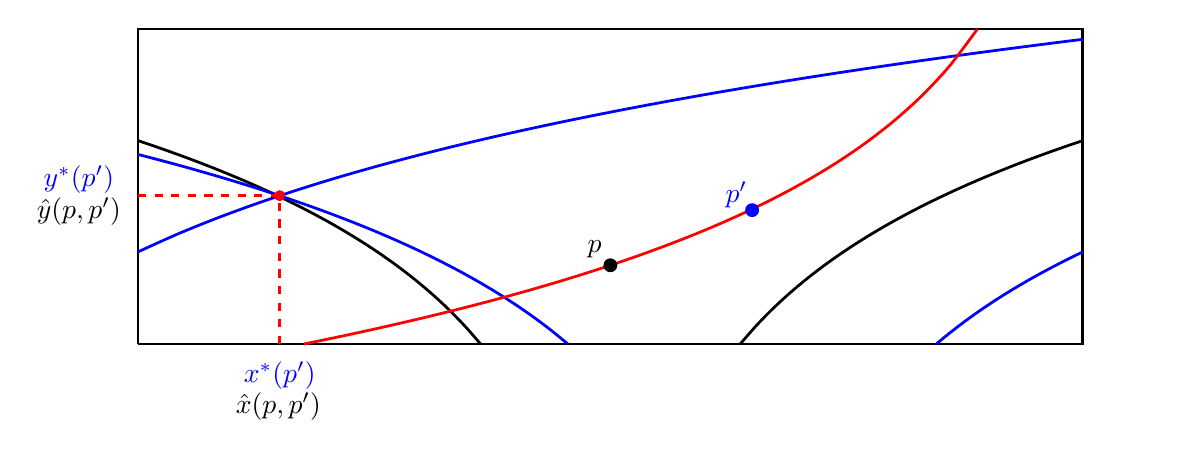
\begin{tikzpicture}
	%Define the coordinates 
	%p = (\u,\v) and p^\prime = (\uu, \vv)
	%Box \Rcal has width 2\r and height \t
	\pgfmathsetmacro{\u}{0}
	\pgfmathsetmacro{\v}{1}
	\pgfmathsetmacro{\uu}{1.8}
	\pgfmathsetmacro{\vv}{1.7}
	\pgfmathsetmacro{\r}{6}
	\pgfmathsetmacro{\t}{4}
	
	%The box \Rcal
	\draw[line width=1pt] (-\r,0) -- (\r,0) -- (\r,\t) -- (-\r,\t) -- (-\r,0);	
	
	%Boundaries p = (\u,\v)
	
	%Right boundary
	\pgfmathsetmacro{\rightbounduv}{\u+exp((\v)/2)}
	\draw[domain=\rightbounduv:\r,smooth,variable=\x,black,line width=1pt] plot (\x, {2*ln(\x)-\v});
    %Left boundary
    \pgfmathsetmacro{\leftbounduv}{\u-exp((\v)/2)}
    \draw[domain=\leftbounduv:-\r,smooth,variable=\x,black,line width=1pt] plot (\x, {2*ln(-\x)-\v});
    
    %Boundaries p^\prime = (\uu,\vv)
    
    %Right boundary
    \pgfmathsetmacro{\rightbounduuvv}{\uu+exp((\vv)/2)}
    \draw[domain=\rightbounduuvv:\r,smooth,variable=\x,blue,line width=1pt] plot (\x, {2*ln(\x-\uu)-\vv});
    %Shifted right boundary
    \pgfmathsetmacro{\shiftrightbounduuvv}{\uu+exp((\vv + \t)/2)-2*\r}
    %\draw[domain=\shiftrightbounduuvv:-\r,smooth,variable=\x,blue,line width=1pt] plot (\x, {2*ln(\x+(2*\r-\uu))-\vv});
    \draw[domain=-\r:\r,smooth,variable=\x,blue,line width=1pt] plot (\x, {2*ln(\x+(2*\r-\uu))-\vv});
    %Left boundary 
    \pgfmathsetmacro{\leftbounduuvv}{\uu-exp((\vv)/2)}
    \draw[domain=\leftbounduuvv:-\r,smooth,variable=\x,blue,line width=1pt] plot (\x, {2*ln(\uu-\x)-\vv});
    %Shifted left boundary

    
    %Star boundary
    \pgfmathsetmacro{\starleftbound}{\r*(1-exp(\v/2))}
    \pgfmathsetmacro{\starrightbound}{\r*(1-exp((\v-\t)/2))}
    \draw[domain=\starleftbound:\starrightbound,smooth,variable=\x,red, line width=1pt] plot (\x, {2*ln((\r/(\r-\x)))+\v});
    
    %Define h_1(p) = h_2(p)
    \pgfmathsetmacro{\hp}{2*ln(\r-\u)-\v}
%    \draw node at (\r+0.75,\hp) {\color{black}$h(y)$};
    \draw node at (\r+1,\hp) {};
    
    %Define h_1(p^\prime) and h_2(p^\prime)
    \pgfmathsetmacro{\hh}{2*ln(\uu+\r)-\vv}
    \pgfmathsetmacro{\hhh}{2*ln(\r-\uu)-\vv}

%    \draw node at (-\r-0.75,\hh+0.1) {\color{blue}$h_1(p^\prime)$};
%    \draw node at (\r+0.75,\hhh) {\color{blue}$h_2(p^\prime)$};
    
    %Define x^\ast(p^\prime) and y^\ast(p^\prime), intersection of left and shifted right blue curve
    \pgfmathsetmacro{\uuast}{\uu-\r}
    \pgfmathsetmacro{\vvast}{2*ln(\r)-\vv}

    %Define intersection left black and shifted blue curve
    \pgfmathsetmacro{\vast}{2*ln((2*\r - \uu)/(exp(\v/2) + exp(\vv/2)))}
    \pgfmathsetmacro{\uast}{(\uu - 2*\r)/(1 + exp((\vv - \v)/2))} 

%    \draw[dashed,thick,black] (-\r,\hhh) -- (\r,\hhh);
    \draw[dashed,line width=1pt,red] (\uuast,0) -- (\uuast,\vvast);
    \draw node at (\uuast,-0.4) {\color{blue}$x^\ast(p^\prime)$};
    \draw[dashed,line width=1pt,red] (-\r,\vvast) -- (\uuast,\vvast);
    \draw node at (-\r-0.75,\vvast+0.2) {\color{blue}$y^\ast(p^\prime)$};
%    \draw[dashed,black,line width=1pt] (-\r,\vast) -- (\uast,\vast);
    \draw node at (-\r-0.75,\vast-0.2) {\color{black}$\hat{y}(p,p^\prime)$};
%    \draw[dashed,black,line width=1pt] (\uast,\vast) -- (\uast,0);
    \draw node at (\uast,-0.8) {\color{black}$\hat{x}(p,p^\prime)$};
    
    \draw node[fill, circle, inner sep=0pt, minimum size=4pt, red] at (\uuast,\vvast) {};
    
   	%Draw both nodes
    \draw node[fill, circle, inner sep=0pt, minimum size=5pt] (p1) at (\u,\v) {};
    \path (p1)+(-0.2,0.2) node {$p$};
    \draw node[fill,blue, circle, inner sep=0pt, minimum size=5pt] (p2) at (\uu,\vv) {};
    \path (p2)+(-0.2,0.2) node {\color{blue}$p^\prime$};
    
    
    
%    \draw node[fill, circle, inner sep=0pt, minimum size=4pt, black] at (\uast,\vast) {};
    
%    \draw node at (-7,2.5835) {$h(y)$};

    
%    \draw[dotted,thick,black] (4.5208,2.0174) -- (4.5208,0);
%    \draw[dotted,thick,black] (4.5208,2.0174) -- (6,2.0174);
    
%    \draw node at (4.5208,-0.5) {$w_x(p,p^\prime)$};
%    \draw node at (7,2.0174) {$w_y(p,p^\prime)$};
    
%    \draw node at (0,3.5) {\color{blue}$x_1 = x^\prime + e^{\frac{y^\prime + y_1}{2}}$};
%    \draw node at (-2,1.6) {\color{blue}$x_1 = x^\prime - e^{\frac{y^\prime + y_1}{2}}$};
%    \draw node at (-4.5,1) {$x_1 = x - e^{\frac{y + y_1}{2}}$};
%    \draw node at (2,1.5) {$x_1 = x + e^{\frac{y + y_1}{2}}$};

\end{tikzpicture}
\caption{Example for a given $p$ of the boundary function $x^\prime \mapsto b^\ast_p(x^\prime)$, given by the red curve, which determines whether $\mathcal{T}(p,p^\prime) = \emptyset$. We see that when $y^\prime = b^\ast_p(x^\prime)$ then $(\hat{x}(p,p^\prime), \hat{y}(p,p^\prime)) = (x^\ast(p^\prime), y^\ast(\prime))$.}
\label{fig:comparing_triangles_diff_analysis}
\end{figure}

This analysis allows us to compute the expected difference in the number of triangles for the finite box model and the infinite model, for a typical node with height $y$, i.e. prove Lemma~\ref{lem:clustering_error_T_term}. 

\begin{figure}[!t]

\centering
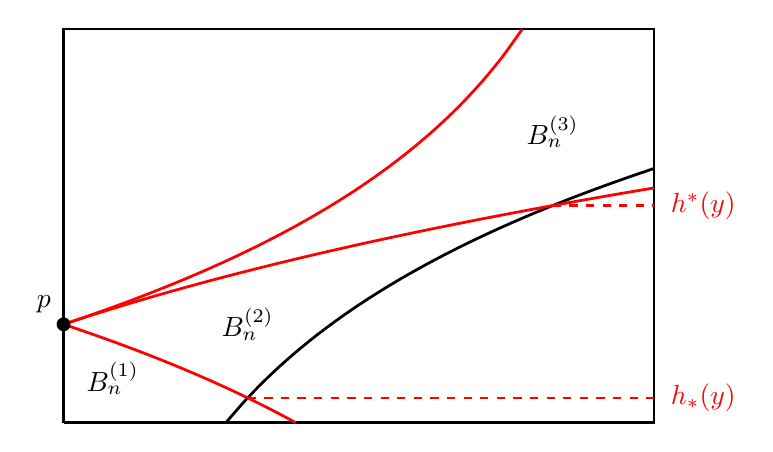
\begin{tikzpicture}[scale=1.25]

%%%%%%%%%%%%%%%%%%%%%%%%%%%%%%%%%%%%%%%%%%%%%%%%%%%%%%%%%%%%%%%%%%%%%%%%%%%%%%%%%%%%%%%%%%%%%%%%%%%
%																								  %
%	Shows the three different areas B_n^{(i)} for the computations in Lemma 					  %
%	\label{lem:clustering_error_T_term}			  												  %
%																								  %
%%%%%%%%%%%%%%%%%%%%%%%%%%%%%%%%%%%%%%%%%%%%%%%%%%%%%%%%%%%%%%%%%%%%%%%%%%%%%%%%%%%%%%%%%%%%%%%%%%%

	%Define the coordinates 
	%p = (\u,\v) and p^\prime = (\uu, \vv)
	%Box \Rcal has width 2\r and height \t
	\pgfmathsetmacro{\u}{0}
	\pgfmathsetmacro{\v}{1}
	\pgfmathsetmacro{\uu}{1.8}
	\pgfmathsetmacro{\vv}{1.7}
	\pgfmathsetmacro{\r}{6}
	\pgfmathsetmacro{\t}{4}
	
	%The box \Rcal only positive x
	\draw[line width=1pt] (0,0) -- (\r,0) -- (\r,\t) -- (0,\t) -- (0,0);	
	
	%Boundaries p = (\u,\v)
	
	%Right boundary
	\pgfmathsetmacro{\rightbounduv}{\u+exp((\v)/2)}
	\draw[domain=\rightbounduv:\r,smooth,variable=\x,black,line width=1pt] plot (\x, {2*ln(\x)-\v});
    %Left boundary
%    \pgfmathsetmacro{\leftbounduv}{\u-exp((\v)/2)}
%    \draw[domain=\leftbounduv:-\r,smooth,variable=\x,black,line width=1pt] plot (\x, {2*ln(-\x)-\v});
    
    %Three boundaries for the regions B_n
    \pgfmathsetmacro{\bone}{\r*(1-exp(-\v/2))}
    \pgfmathsetmacro{\btwo}{\r*(exp(-\v/2)-1)}
    %Star boundary
    \pgfmathsetmacro{\bthreeleft}{\r*(1-exp(\v/2))}
    \pgfmathsetmacro{\bthreeright}{\r*(1-exp((\v-\t)/2))}
    
    \draw[domain=0:\bone,smooth,variable=\x,red,line width=1pt] plot (\x, {\v-2*ln(\r/(\r-\x))});
    \draw[domain=0:\r,smooth,variable=\x,red,line width=1pt] plot (\x, {\v+2*ln(1+(\x/\r))});
    \draw[domain=0:\bthreeright,smooth,variable=\x,red, line width=1pt] plot (\x, {2*ln((\r/(\r-\x)))+\v});    
    
    %Define the top and bottom coordinates of y^prime boundaries
    \pgfmathsetmacro{\ybottom}{\v+2*ln(\r/(\r+exp(\v)))}
    \pgfmathsetmacro{\xbottom}{\r*exp(\v)/(\r + exp(\v))}
    \pgfmathsetmacro{\ytop}{\v+2*ln(\r/(\r-exp(\v)))}
    \pgfmathsetmacro{\xtop}{\r*exp(\v)/(\r - exp(\v))}
    
    \draw[dashed,line width=1pt,red] (\xbottom,\ybottom) -- (\r,\ybottom);
    \draw[dashed,line width=1pt,red] (\xtop,\ytop) -- (\r,\ytop);
    \draw node at (\r+0.5,\ybottom) {\color{red}$h_\ast(y)$};
    \draw node at (\r+0.5,\ytop) {\color{red}$h^\ast(y)$};
    
    \draw node at (0.5,\ybottom+0.2) {$B_n^{(1)}$};
    \draw node at (\xbottom,\ybottom+0.75) {$B_n^{(2)}$};
    \draw node at (\xtop,\ytop+0.75) {$B_n^{(3)}$};
    

    %Define h_1(p) = h_2(p)
    \pgfmathsetmacro{\hp}{2*ln(\r-\u)-\v}
  
    %Define h_1(p^\prime) and h_2(p^\prime)
    \pgfmathsetmacro{\hh}{2*ln(\uu+\r)-\vv}
    \pgfmathsetmacro{\hhh}{2*ln(\r-\uu)-\vv}

%    \draw node at (-\r-0.75,\hh+0.1) {\color{blue}$h_1(p^\prime)$};
%    \draw node at (\r+0.75,\hhh) {\color{blue}$h_2(p^\prime)$}; 
    
   	%Draw node p
    \draw node[fill, circle, inner sep=0pt, minimum size=5pt] (p1) at (\u,\v) {};
    \path (p1)+(-0.2,0.2) node {$p$};

\end{tikzpicture}
\caption{Three different areas $B_n^{(i)}$ used in the proof of Lemma \ref{lem:clustering_error_T_term}.}
\label{fig:comparing_triangles_B_areas}
\end{figure}

\begin{proof}[Proof of Lemma \ref{lem:clustering_error_T_term}]
Due to symmetry it is enough to show that
\begin{equation}\label{eq:clustering_error_T_main}
	\int_0^{R_n}\int_0^{I_n} \mu\left(\mathcal{T}(p,p^\prime)(p,p_1)\right) f(x_1,y_1) 
	\dd x_1 \dd y_1 = \bigO{y n^{-(2\alpha - 1)} + n^{-(2\alpha-1)} e^{y}}
\end{equation}
The proof goes in two stages. First we compute $\mu\left(\mathcal{T}(p,p^\prime)(p,p_1)\right)$ by splitting it over three disjoint regimes with respect to $p_1$, with $x_1 \ge 0$. Then we do the integration with respect to $p_1$.

\subsubsection*{Computing $\bm{\mu\left(\mathcal{T}(p,p^\prime)(p,p_1)\right)}$}

Recall that $I_n = \frac{\pi}{2} e^{R_n/2}$ and define the sets
\begin{align*}
	A_n^{(1)} &= \left\{p_1 = (x_1,y_1) \in \Rcal \, : \, 0 \le y_1 \le y - 2\log(I_n/(I_n-x_1)) \right\},\\
	A_n^{(2)} &= \left\{p_1 = (x_1,y_1) \in \Rcal \, : \, y - 2\log(I_n/(I_n-x_1)) < y_1 
		\le y + 2 \log\left(1 + \frac{x_1}{I_n}\right)\right\},\\
	A_n^{(3)} &= \left\{p_1 = (x_1,y_1) \in \Rcal \, : \, y + 2 \log\left(1 + \frac{x_1}{I_n}\right) < y_1 
			\le y + 2 \log\left(\frac{I_n}{I_n-x_1}\right)\right\},
\end{align*}
and let $B_n^{(i)} = \BallPon{p} \cap A_n^{(i)}$, for $i = 1, 2, 3$, see Figure~\ref{fig:comparing_triangles_B_areas}. Here the heights of the two intersections are given by
\begin{align}
	h_\ast(y) &= y + 2 \log\left(\frac{I_n}{I_n + e^y}\right)\\
	h^\ast(y) &= y + 2 \log\left(\frac{I_n}{I_n - e^y}\right).
\end{align}

With these definitions we have that the union $B_n := \bigcup_{i = 1}^n B_n^{(i)}$ denotes the area under the red curve in Figure~\ref{fig:comparing_triangles_diff_analysis} and hence, for all $p_1 \in \Rcal\setminus B_n$ with $x_1 \ge 0$ we have that $\mathcal{T}(p,p^\prime)(p,p_1) = \emptyset$. So we only need to consider $p_1 \in B_n$. We shall establish the following result:
\begin{equation}\label{eq:mu_triangle_diff}
	\mu\left(\mathcal{T}(p,p^\prime)(p,p_1)\right) = 
	\begin{cases}
		\bigO{I_n^{-2\alpha} e^{\alpha y_1}} &\mbox{if } p_1 \in B_n^{(1)}\\
		\bigO{I_n^{-2\alpha} e^{\alpha y}} &\mbox{if } p_1 \in B_n^{(2)} \cup B_n^{(3)}
	\end{cases}
\end{equation}

Depending on which set $p_1$ belongs to, the set $\mathcal{T}(p,p^\prime)(p,p_1)$ has a different shape. We displayed these shapes in Figure~\ref{fig:shapes_triangle_mismatches} as a visual aid to follow the computations below. 

\begin{figure}[!tp]
\centering
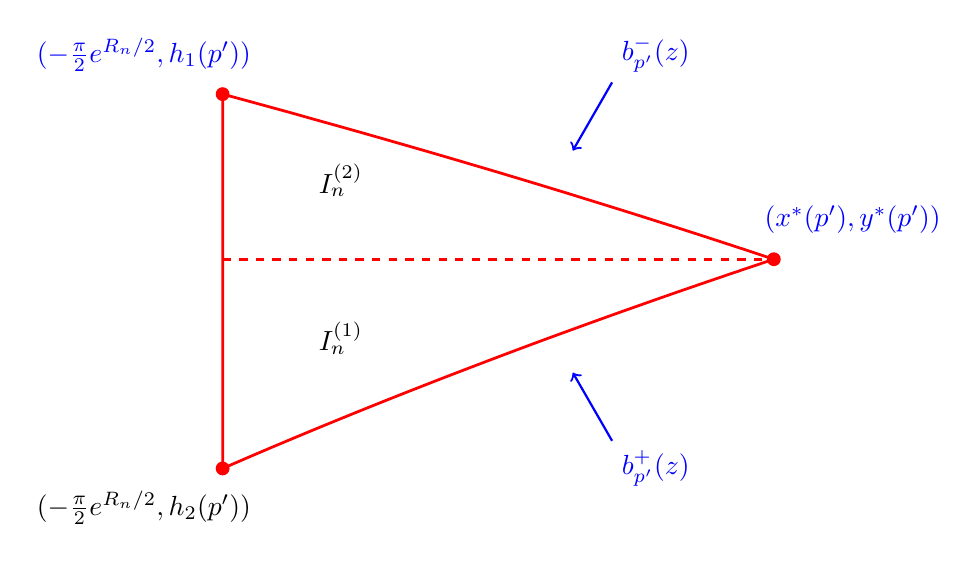
\begin{tikzpicture}[scale=5]

%%%%%%%%%%%%%%%%%%%%%%%%%%%%%%%%%%%%%%%%%%%%%%%%%%%%%%%%%%%%%%%%%%%%%%%%%%%%%%%%%%%%%%%%%%%%%%%%%%%
%																								  %
%	Shows the area T_{\Pcal \Delta \Pcal} when h_1(p^\prime) > h_2(p^\prime) > h(y)			  %
%																								  %
%%%%%%%%%%%%%%%%%%%%%%%%%%%%%%%%%%%%%%%%%%%%%%%%%%%%%%%%%%%%%%%%%%%%%%%%%%%%%%%%%%%%%%%%%%%%%%%%%%%

	%Define the coordinates 
	%p = (\u,\v) and p^\prime = (\uu, \vv)
	%Box \Rcal has width 2\r and height \t
	\pgfmathsetmacro{\u}{0}
	\pgfmathsetmacro{\v}{1}
	\pgfmathsetmacro{\uu}{1.4}
	\pgfmathsetmacro{\vv}{0.2}
	\pgfmathsetmacro{\r}{6}
	\pgfmathsetmacro{\t}{4}
    
    %Define x^\ast(p^\prime) and y^\ast(p^\prime)
    \pgfmathsetmacro{\uuast}{\uu-\r}
    \pgfmathsetmacro{\vvast}{2*ln(\r)-\vv}
    
    %Define intersection left black and shifted blue curve
    \pgfmathsetmacro{\vast}{2*ln((2*\r - \uu)/(exp(\v/2) + exp(\vv/2)))}
    \pgfmathsetmacro{\uast}{(\uu - 2*\r)/(1 + exp((\vv - \v)/2))}    
   
    %Define h_1(p) = h_2(p)
    \pgfmathsetmacro{\hp}{2*ln(\r-\u)-\v}
    
    %Define h_1(p^\prime) and h_2(p^\prime)
    \pgfmathsetmacro{\hh}{2*ln(\uu+\r)-\vv}
    \pgfmathsetmacro{\hhh}{2*ln(\r-\uu)-\vv}
    
    %Draw the boundary left black, left blue and shifted right blue line
	\draw[red,line width=1pt] 
		plot[domain=\uuast:-\r,smooth,variable=\x,red] (\x, {2*ln(\x+(2*\r-\uu))-\vv}) 
		-- 
		(-\r,\hh)
		-- 
		plot[domain=-\r:\uuast,smooth,variable=\x,red] (\x, {2*ln(\uu-\x)-\vv});
	
	\pgfmathsetmacro{\top}{2*ln(\uu-\uast)-\vv}
	
	\draw[red, dashed,line width=1pt] (-\r,\vvast) -- (\uuast,\vvast);

    \draw node at (-\r-0.2,\hh+0.1) {\color{blue}$(-\frac{\pi}{2} e^{R_n/2}, h_1(p^\prime))$};
    \draw node at (-\r-0.2,\hhh-0.1) {$(-\frac{\pi}{2} e^{R_n/2}, h_2(p^\prime))$};
    \draw node at (\uuast+0.2,\vvast+0.1) {\color{blue}$(x^\ast(p^\prime), y^\ast(p^\prime))$};
    
    \draw node at (-\r+0.3,\vvast+0.2) {$I_n^{(2)}$};
    \draw node at (-\r+0.3,\vvast-0.2) {$I_n^{(1)}$};
    
    \draw node (f2) at (\uuast-0.3,\hh+0.1) {\color{blue}$b_{p^\prime}^-(z)$};
    \draw node (f3) at (\uuast-0.3,\hhh) {\color{blue}$b_{p^\prime}^+(z)$};
    \path (f2)+(230:0.35) node (f2_arrow) {};
    \path (f3)+(130:0.35) node (f3_arrow) {};
    \draw[->,thick,blue] (f2.south west) -- (f2_arrow);
    \draw[->,thick,blue] (f3.north west) -- (f3_arrow);

	\draw node[red, fill, circle, inner sep=0pt, minimum size=5pt] at (-\r,\hhh) {};
	\draw node[red, fill, circle, inner sep=0pt, minimum size=5pt] at (-\r,\hh) {};
	\draw node[red, fill, circle, inner sep=0pt, minimum size=5pt] at (\uuast,\vvast) {};

\end{tikzpicture}\\
\vspace{20pt}
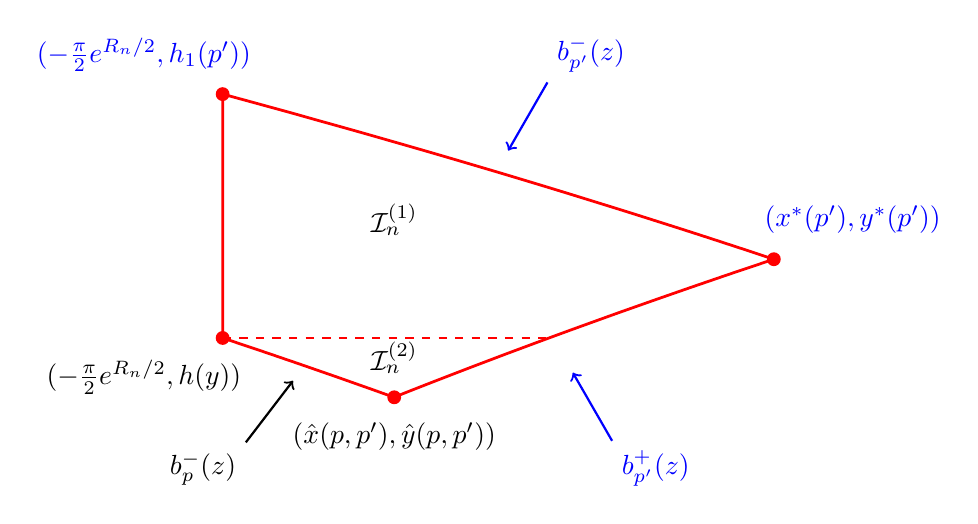
\begin{tikzpicture}[scale=5]
	%Define the coordinates 
	%p = (\u,\v) and p^\prime = (\uu, \vv)
	%Box \Rcal has width 2\r and height \t
	\pgfmathsetmacro{\u}{0}
	\pgfmathsetmacro{\v}{1}
	\pgfmathsetmacro{\uu}{1.4}
	\pgfmathsetmacro{\vv}{0.8}
	\pgfmathsetmacro{\r}{6}
	\pgfmathsetmacro{\t}{4}
    
    %Define x^\ast(p^\prime) and y^\ast(p^\prime)
    \pgfmathsetmacro{\uuast}{\uu-\r}
    \pgfmathsetmacro{\vvast}{2*ln(\r)-\vv}
    
    %Define intersection left black and shifted blue curve
    \pgfmathsetmacro{\vast}{2*ln((2*\r - \uu)/(exp(\v/2) + exp(\vv/2)))}
    \pgfmathsetmacro{\uast}{(\uu - 2*\r)/(1 + exp((\vv - \v)/2))}    
   
    %Define h_1(p) = h_2(p)
    \pgfmathsetmacro{\hp}{2*ln(\r-\u)-\v}
    
    %Define h_1(p^\prime) and h_2(p^\prime)
    \pgfmathsetmacro{\hh}{2*ln(\uu+\r)-\vv}
    \pgfmathsetmacro{\hhh}{2*ln(\r-\uu)-\vv}
    
    %Draw the boundary left black, left blue and shifted right blue line
	\draw[red,line width=1pt] 
		plot[domain=\uuast:\uast,smooth,variable=\x,red] (\x, {2*ln(\x+(2*\r-\uu))-\vv}) 
		-- 
		plot[domain=\uast:-\r,smooth,variable=\x,red] (\x, {2*ln(-\x)-\v})
		-- 
		(-\r,\hh)
		-- 
		plot[domain=-\r:\uuast,smooth,variable=\x,red] (\x, {2*ln(\uu-\x)-\vv});
	
	\pgfmathsetmacro{\rb}{\uu + exp((\vv+\hp)/2) -2*\r}
	

	%\draw[red,dashed,line width=1pt] (\uast,\vast) -- (\uast,\hp);
	\draw[red,dashed,line width=1pt] (-\r,\hp) -- (\rb,\hp);

    \draw node at (-\r-0.2,\hh+0.1) {\color{blue}$(-\frac{\pi}{2} e^{R_n/2}, h_1(p^\prime))$};
    \draw node at (-\r-0.2,\hp-0.1) {$(-\frac{\pi}{2} e^{R_n/2}, h(y))$};
    \draw node at (\uuast+0.2,\vvast+0.1) {\color{blue}$(x^\ast(p^\prime), y^\ast(p^\prime))$};
    \draw node at (\uast,\vast-0.1) {$(\hat{x}(p,p^\prime), \hat{y}(p, p^\prime))$};
    
    \draw node at (\uast,\vvast+0.1) {$\mathcal{I}_n^{(1)}$};
    \draw node at (\uast,\hp-0.05) {$\mathcal{I}_n^{(2)}$};
    %\draw node at (\uast+0.1,\hp-0.05) {$\mathcal{I}_n^{(3)}$};
    
    \draw node (f1) at (-\r-0.05,\hhh) {$b_p^-(z)$};
    \draw node (f2) at (\uast+0.5,\hh+0.1) {\color{blue}$b_{p^\prime}^-(z)$};
    \draw node (f3) at (\uuast-0.3,\hhh) {\color{blue}$b_{p^\prime}^+(z)$};
    \path (f1)+(45:0.35) node (f1_arrow) {};
    \path (f2)+(230:0.35) node (f2_arrow) {};
    \path (f3)+(130:0.35) node (f3_arrow) {};
    \draw[->,thick] (f1.north east) -- (f1_arrow);
    \draw[->,thick,blue] (f2.south west) -- (f2_arrow);
    \draw[->,thick,blue] (f3.north west) -- (f3_arrow);

	\draw node[red, fill, circle, inner sep=0pt, minimum size=5pt] at (-\r,\hp) {};
	\draw node[red, fill, circle, inner sep=0pt, minimum size=5pt] at (-\r,\hh) {};
	\draw node[red, fill, circle, inner sep=0pt, minimum size=5pt] at (\uuast,\vvast) {};
	\draw node[red, fill, circle, inner sep=0pt, minimum size=5pt] at (\uast,\vast) {};

\end{tikzpicture}\\
\vspace{20pt}
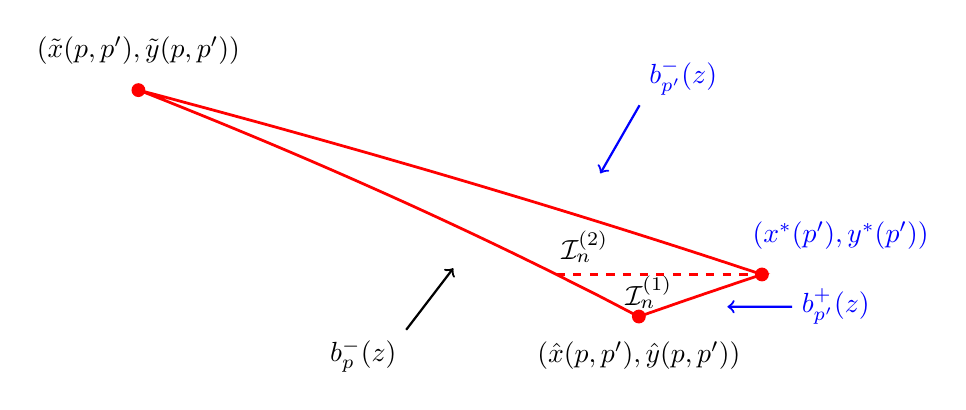
\begin{tikzpicture}[scale=5]

%%%%%%%%%%%%%%%%%%%%%%%%%%%%%%%%%%%%%%%%%%%%%%%%%%%%%%%%%%%%%%%%%%%%%%%%%%%%%%%%%%%%%%%%%%%%%%%%%%%
%																								  %
%	Shows the area T_{\Pcal \Delta \Pcal} when h(y) > h_1(p^\prime)							  %
%																								  %
%%%%%%%%%%%%%%%%%%%%%%%%%%%%%%%%%%%%%%%%%%%%%%%%%%%%%%%%%%%%%%%%%%%%%%%%%%%%%%%%%%%%%%%%%%%%%%%%%%%

	%Define the coordinates 
	%p = (\u,\v) and p^\prime = (\uu, \vv)
	%Box \Rcal has width 2\r and height \t
	\pgfmathsetmacro{\u}{0}
	\pgfmathsetmacro{\v}{1}
	\pgfmathsetmacro{\uu}{2.5}
	\pgfmathsetmacro{\vv}{1.8}
	\pgfmathsetmacro{\r}{6}
	\pgfmathsetmacro{\t}{4}
    
    %Define x^\ast(p^\prime) and y^\ast(p^\prime)
    \pgfmathsetmacro{\uuast}{\uu-\r}
    \pgfmathsetmacro{\vvast}{2*ln(\r)-\vv}
    
    %Define intersection left black and shifted blue curve
    \pgfmathsetmacro{\vast}{2*ln((2*\r - \uu)/(exp(\v/2) + exp(\vv/2)))}
    \pgfmathsetmacro{\uast}{(\uu - 2*\r)/(1 + exp((\vv - \v)/2))}    
    
    %Define intersection left black and left blue curve
    \pgfmathsetmacro{\utilde}{\uu/(1-exp((\vv-\v)/2))} 
    \pgfmathsetmacro{\vtilde}{2*ln(\uu-\utilde)-\vv}
   
    %Define h_1(p) = h_2(p)
    \pgfmathsetmacro{\hp}{2*ln(\r-\u)-\v}
    
    %Define h_1(p^\prime) and h_2(p^\prime)
    \pgfmathsetmacro{\hh}{2*ln(\uu+\r)-\vv}
    \pgfmathsetmacro{\hhh}{2*ln(\r-\uu)-\vv}
    
    %Draw the boundary left black, left blue and shifted right blue line
	\draw[red,line width=1pt] 
		plot[domain=\utilde:\uuast,smooth,variable=\x,red] (\x, {2*ln(\uu-\x)-\vv})
		--
		plot[domain=\uuast:\uast,smooth,variable=\x,red] (\x, {2*ln(\x+(2*\r-\uu))-\vv})
		--
		plot[domain=\uast:\utilde,smooth,variable=\x,red] (\x, {2*ln(-\x)-\v}); 
	
	%Calculate intersection point
	\pgfmathsetmacro{\i}{-exp((\v+\vvast)/2)}
	\draw[red, dashed,line width=1pt] (\i,\vvast) -- (\uuast,\vvast);

    \draw node at (\utilde,\vtilde+0.1) {\color{black}$(\tilde{x}(p,p^\prime), \tilde{y}(p,p^\prime))$};
    \draw node at (\uast,\vast-0.1) {$(\hat{x}(p,p^\prime), \hat{y}(p,p^\prime))$};
    \draw node at (\uuast+0.2,\vvast+0.1) {\color{blue}$(x^\ast(p^\prime), y^\ast(p^\prime))$};
   
    \draw node at (\uuast-0.45,\vvast+0.07) {$\mathcal{I}_n^{(2)}$};
    \draw node at (\uast+0.025,\vvast-0.045) {$\mathcal{I}_n^{(1)}$};
   
    \draw node (f1) at (\uast-0.7,\vast-0.1) {\color{black}$b_{p}^-(z)$};
    \draw node (f2) at (\uuast-0.2,\vvast+0.5) {\color{blue}$b_{p^\prime}^-(z)$};
    \draw node (f3) at (\uast+0.5,\vast+0.025) {\color{blue}$b_{p^\prime}^+(z)$};
    \path (f1)+(45:0.35) node (f1_arrow) {};
    \path (f2)+(230:0.35) node (f2_arrow) {};
    \path (f3)+(180:0.3) node (f3_arrow) {};
	\draw[->,thick] (f1.north east) -- (f1_arrow);
    \draw[->,thick,blue] (f2.south west) -- (f2_arrow);
    \draw[->,thick,blue] (f3.west) -- (f3_arrow);
%
	\draw node[red, fill, circle, inner sep=0pt, minimum size=5pt] at (\utilde,\vtilde) {};
	\draw node[red, fill, circle, inner sep=0pt, minimum size=5pt] at (\uast,\vast) {};
	\draw node[red, fill, circle, inner sep=0pt, minimum size=5pt] at (\uuast,\vvast) {};

\end{tikzpicture}
\caption{The different shapes of $\mathcal{T}(p,p^\prime)(p,p_1)$ depending on the regime to which $p_1$ belongs. The top figure is for $p_1 \in B_n^{(1)}$, the middle for $p_1 \in B_n^{(2)}$ and the bottom one for $p_1 \in B_n^{(3)}$.}
\label{fig:shapes_triangle_mismatches}
\end{figure}

\paragraph{Regime 1: $0 \le y_1 \le y - 2\log(I_n/(I_n-x_1))$}

In this case the integral over $p_2$ splits into two parts
\begin{align*}
	\mathcal{I}_n^{(1)}(p_1) &:= \int_{h_2(p_1)}^{y^\ast(p_1)} \int_{-I_n}^{x_1 + e^{(y_1+y_2)/2}-2I_n} e^{-\alpha y_2}
		\dd x_2 \dd y_2\\
	\mathcal{I}_n^{(2)}(p_1) &:= \int_{y^\ast(p_1)}^{h_1(p_1)} \int_{x^\ast(p_1)}^{x_1 - e^{(y_1+y_2)/2}} e^{-\alpha y_2}
		\dd x_2 \dd y_2.
\end{align*}

We first compute $\mathcal{I}_n^{(1)}$.
\begin{align*}
	\mathcal{I}_n^{(1)}(p_1) &= \int_{h_2(p_1)}^{y^\ast(p_1)} \left(x_1 + e^{(y_1+y_2)/2} - I_n\right) e^{-\alpha y_2} 
		\dd y_2\\
	&\le e^{y_1/2} \int_{h_2(p_1)}^{y^\ast(p_1)} e^{-(\alpha-\frac{1}{2}) y_2} \dd y_2\\
	&= \frac{2 e^{y_1/2}}{2\alpha - 1} \left(e^{-(\alpha-\frac{1}{2})h_2(p_1)} - e^{-(\alpha-\frac{1}{2})y^\ast(p_1)}
		\right) \\
	&= \frac{2 e^{\alpha y_1}}{2\alpha - 1} I_n^{-(2\alpha -1)}\left(\left(1 - \frac{x_1}{I_n}\right)^{-(2\alpha - 1)}-1\right)\\
	&= \bigO{I_n^{-2\alpha} x_1 e^{\alpha y_1}},
\end{align*}
where we used that $x_1 \le e^{(y+y_1)/2} = \smallO{I_n}$ for all $y_1\le y$ and $y \in \Kcal_{C}(k_n)$ so that
\[
	\left(\left(1 - \frac{x_1}{I_n}\right)^{-(2\alpha - 1)}-1\right) = \bigO{\frac{x^\prime}{I_n}} \quad 
	\text{as } n \to \infty.
\]

For $\mathcal{I}_n^{(2)}(p_1)$ we have
\begin{align*}
	\mathcal{I}_n^{(2)}(p_1) &= \int_{y^\ast(p_1)}^{h_1(p_1)} \left(I_n + x_1 - e^{(y_1+y_2)}\right) e^{-\alpha y_2}
		\dd y_2\\
	&\le 2 I_n \int_{y^\ast(p_1)}^{h_1(p_1)} e^{-\alpha y_2} \dd x_2 \dd y_2\\
	&= \frac{2}{\alpha} I_n \left(I_n^{-2\alpha}e^{\alpha y_1} - \left(I_n + x_1\right)^{-2\alpha} e^{-\alpha y_1}\right)\\
	&= \bigO{I_n^{-2\alpha} x_1 e^{\alpha y_1}} = \bigO{I_n^{-(2\alpha - 1)} e^{\alpha y_1}}.
\end{align*}

We conclude that for $p_1 \in B_n^{(1)}$:
\[
	\mu\left(\mathcal{T}(p,p^\prime)(p,p_1)\right) = \bigO{I_n^{-2\alpha} x_1 e^{\alpha y_1}},
\]
which establishes the first part of \eqref{eq:mu_triangle_diff}.

\paragraph{Regime 2: $y - 2\log(I_n/(I_n-x_1)) < y_1 \le y + 2 \log\left(1 + \frac{x_1}{I_n}\right)$}

Here we split the integration into two parts (see Figure~\ref{fig:shapes_triangle_mismatches}). Recall that $x^\ast(p,p_1) = x_1 - I_n$. Then, for the first part we have
\begin{align*}
	\mathcal{I}_n^{(1)}(p,p_1) &\le \int_{h(y)}^{h_1(p_1)} \int_{-I_n}^{x^\ast(p,p_1)} f(x_2, y_2) 
		\dd x_2 \dd y_2\\
	&= \bigO{x_1 \left(e^{-\alpha h(y)} - e^{-\alpha h_1(p_1)}\right)}\\
	&= \bigO{x_1 I_n^{-2\alpha}\left(e^{\alpha y} - e^{\alpha y_1}\left(1 + \frac{x_1}{I_n}\right)^{-2\alpha}\right)}\\
	&= \bigO{I_n^{-2\alpha} x_1 e^{\alpha y_1}\left(\left(1 - \frac{x_1}{I_n}\right)^{-2\alpha} 
		- \left(1 + \frac{x_1}{I_n}\right)^{-2\alpha}\right)}\\
	&= \bigO{I_n^{-2\alpha} x_1 e^{\alpha y_1}} = \bigO{I_n^{-(2\alpha - 1)} e^{\alpha y}}, 
\end{align*}
were we used that $y \le y_1 + 2\log(I_n/(I_n-x_1))$ for $p_1 \in B_n^{(2)}$ for the third line and 
\[
	\left(1 - \frac{x_1}{I_n}\right)^{-2\alpha} - \left(1 + \frac{x_1}{I_n}\right)^{-2\alpha}
	= \bigO{\frac{x_1}{I_n}} = \bigO{1},
\]
for the last line.

For the second part we first compute that 
\begin{align*}
	x_1 + e^{(y_1+y_2)/2} - 2 I_n + e^{(y + y_2)/2} &\le \left(e^{y/2} + e^{y_1/2}\right)e^{y_2/2}\\
	&\le e^{y/2}\left(1 + \frac{I_n}{I_n - e^y}\right)e^{y_2/2} = \bigO{e^{(y+y_2)/2}},
\end{align*}
since $y \in \Kcal_{C}(k_n)$ and $k_n = \smallO{\sqrt{n}}$, so that $e^y = \smallO{n} = \smallO{I_n}$. 
Then we have
\begin{align*}
	\mathcal{I}_n^{(2)} &= \int_{\hat{y}(p,p_1)}^{h(y)} \int_{-e^{(y + y_2)/2}}^{x_1 + e^{(y+y_1)/2} - 2 I_n} 
		f(x_2, y_2) \dd x_2 \dd y_2\\
	&= \bigO{e^{y/2} \int_{\hat{y}(p,p_1)}^{h(y)} e^{-(\alpha -\frac{1}{2}) y_2} \dd y_2}\\
	&= \bigO{e^{y/2} \left(e^{-(\alpha -\frac{1}{2}) \hat{y}(p,p_1)} - e^{-(\alpha -\frac{1}{2}) h(y)}\right)}\\
	&= \bigO{e^{y/2} \left(\left(\frac{2I_n - x_1}{e^{y/2} + e^{y_1/2}}\right)^{-(2\alpha-1)} 
		- I_n^{-(2\alpha-1)} e^{(\alpha -\frac{1}{2}) y}\right)}\\
	&= \bigO{I_n^{-(2\alpha-1)} e^{\alpha y}},
\end{align*}
where for the last line we first used that $(2I_n - x_1)^{-(2\alpha-1)} \le I_n^{-(2\alpha-1)}$ and then
\[
	\left(\left(e^{y/2} + e^{y_1/2}\right)^{2\alpha-1}- e^{(\alpha -\frac{1}{2}) y}\right)
	\le e^{(\alpha -\frac{1}{2}) y}\left(\left(1 + \sqrt{1+\frac{x_1}{I_n}} \, \right)^{2\alpha - 1} - 1\right)
	= \bigO{e^{(\alpha -\frac{1}{2}) y}}.
\]

It then follows that for $p_1 \in B_n^{(2)}$
\[
	\mu\left(\mathcal{T}(p,p^\prime)(p,p_1)\right) = \bigO{I_n^{-(2\alpha-1)} e^{\alpha y}}.
\]

\paragraph{Regime 3:}

\begin{align*}
	\mathcal{I}_n^{(1)} &= \int_{y^\ast}^{\tilde{y}} \int_{-e^{(y+y_2)/2}}^{x_1-e^{(y_1+y_2)/2}} f(x_2,y_2)
		\dd x_2 \dd y_2\\
	&= \bigO{\int_{y^\ast}^{\tilde{y}} x_1 e^{-\alpha y_2} - \left(e^{y_1/2} - e^{y/2}\right)e^{-(\alpha - \frac{1}{2})y_2}
		\dd y_2}\\
	&= \bigO{x_1 \int_{y^\ast}^{\tilde{y}}  e^{-\alpha y_2} \dd y_2}.
\end{align*}

Now 
\begin{align*}
	\int_{y^\ast}^{\tilde{y}}  e^{-\alpha y_2} \dd y_2 
	&= \frac{1}{\alpha}\left(e^{-\alpha y^\ast} - e^{-\alpha \tilde{y}}\right) 
		= \frac{1}{\alpha}\left(I_n^{-2\alpha} e^{\alpha y_1} 
		- \left(\frac{x_1}{e^{y_1/2} - e^{y/2}}\right)^{-2\alpha}\right) \\
	&= \frac{I_n^{-2\alpha} e^{\alpha y_1}}{\alpha}\left(1 - \left(1 - e^{(y - y_1)/2}\right)^{2\alpha}
		\left(\frac{x_1}{I_n}\right)^{-2\alpha}\right) = \bigO{I_n^{-2\alpha} e^{\alpha y_1}},
\end{align*}
and hence we have
\[
	\mathcal{I}_n^{(1)} = \bigO{I_n^{-2\alpha} x_1 e^{\alpha y_1}}.
\]

For the second integral we have
\begin{align*}
	\mathcal{I}_n^{(2)} &= \int_{\hat{y}}^{y^\ast} \int_{-e^{(y+y_2)/2}}^{e^{(y_1 + y_2)/2} + x_1 - 2I_n} 
		f(x_2,y_2)\dd x_2 \dd y_2\\
	&= \bigO{\int_{\hat{y}}^{y^\ast} \left(e^{y/2} + e^{y_1/2}\right)e^{-(\alpha - \frac{1}{2})y_2} \dd y_2}\\
	&= \bigO{ e^{y_1/2} \int_{\hat{y}}^{y^\ast}e^{-(\alpha - \frac{1}{2})y_2} \dd y_2}.
\end{align*}

For the integral we have
\begin{align*}
	\int_{\hat{y}}^{y^\ast}e^{-(\alpha - \frac{1}{2})y_2} \dd y_2
	&= \frac{2}{2\alpha - 1} \left(e^{-(\alpha - \frac{1}{2})\hat{y}} - e^{-(\alpha - \frac{1}{2})y^\ast}\right)\\
	&= \frac{2}{2\alpha - 1}\left(\left(\frac{2I_n - x_1}{e^{y/2} + e^{y_1/2}}\right)^{-(2\alpha - 1)} 
		- I_n^{-(2\alpha - 1)} e^{-(\alpha - \frac{1}{2})y_1}\right)\\
	&= \bigO{I_n^{-2\alpha} x_1 e^{-(\alpha - \frac{1}{2})y_1}}
\end{align*}
so that
\[
	\mathcal{I}_n^{(2)} = \bigO{I_n^{-(2\alpha - 1)} e^{(1-\alpha)y_1}} = \bigO{I_n^{-2\alpha} x_1 e^{\alpha y}}
\]
and hence for $p_1 \in B_n^{(3)}$
\[
	\mu\left(\mathcal{T}(p,p^\prime)(p,p_1)\right) = \bigO{I_n^{-2\alpha} x_1 e^{\alpha y}}
	= \bigO{I_n^{-(2\alpha - 1)} e^{\alpha y}}.
\]

\subsubsection*{Integration over $p_1$}



We now proceed with the second part of the computation leading to \eqref{eq:clustering_error_T_main}. Here we will integrate $\mu(\mathcal{T}(p,p^\prime))(p,p_1)$ over the region $B_n := B_n^{(1)} \cup B_n^{(2)} \cup B_n^{(3)}$, see Figure~\ref{fig:comparing_triangles_B_areas}. Let us first identify the boundaries of these areas. 

The area $B_n^{(1)}$ is bounded from above by the line given by the equation
\[
	y_1 = y - 2\log\left(\frac{I_n}{I_n - x_1}\right).
\]
Solving this for $x_1$ yields $x_1 = I_n\left(1 - e^{(y_1-y)/2}\right)$ and hence the area $B_n^{(1)}$ is given by
\[
	B_n^{(1)} = \left\{(x_1, y_1) \, : \, 0 \le y_1 \le y, \quad 0 \le x_1 \le I_n\left(1 - e^{(y_1-y)/2}\right) \wedge e^{(y + y_1)/2} \right\}.
\]

In a similar way we have that $B_n^{(2)}$ is bounded from above by line
\[
	y_1 = y + 2\log\left(\frac{I_n}{I_n + x_1}\right),
\]
which yields $x_1 = I_n\left(e^{(y_1 - y)/2} - 1\right)$. The lower red boundary is the upper boundary of $B_n^{(2)}$ and hence we have
\[
	B_n^{(2)} = \left\{(x_1, y_1) \, : \, h_\ast(y) \le y_1 \le h^\ast(y), \,\, I_n\left(1 - e^{(y_1-y)/2}\right) \vee 
	I_n\left(e^{(y_1 - y)/2} - 1\right) \le x_1 \le e^{(y + y_1)/2} \right\}.
\]

We continue in the same way for $B_n^{(3)}$
\[
	B_n^{(3)} = \left\{(x_1, y_1) \, : \, y \le y_1 \le R_n, \,\,
	I_n\left(1 - e^{(y - y_1)/2}\right) \le x_1 \le I_n\left(e^{(y_1 - y)/2} - 1\right) \wedge e^{(y + y_1)/2} \wedge I_n \right\}.
\]

We these characterizations of the areas we now integrate $\mu(\mathcal{T}(p,p^\prime))(p,p_1)$ over $B_n$, splitting the computations over the three different areas.

\paragraph{$\bm{p_1 \in B_n^{(1)}}:$}

We use that $I_n\left(1 - e^{(y_1-y)/2}\right) \wedge e^{(y + y_1)/2} \le I_n\left(1 - e^{(y_1-y)/2}\right)$ so that
\begin{align*}
	&\hspace{-30pt}\int_{B_n^{(1)}} \mu\left(\mathcal{T}(p,p^\prime)(p,p_1)\right) 
		f(x_1,y_1)	\dd x_1 \dd y_1 \\
	&\le  \int_0^y \int_0^{I_n(1-e^{(y_1-y)/2})} \mu\left(\mathcal{T}(p,p^\prime)(p,p_1)\right) 
		f(x_1,y_1) \dd x_1 \dd y_1\\
	&= \bigO{ I_n^{-2\alpha} \int_0^y \int_0^{e^{(y+y_1)/2}}  x_1 \dd x_1 \dd y_1 }\\
	&= \bigO{I_n^{-(2\alpha-1)} \int_0^y \left(1 - e^{(y_1-y)/2}\right)^2 \dd y_1} \\
	&= \bigO{I_n^{-(2\alpha - 1)} y} = \bigO{y n^{-(2\alpha - 1)}}.
\end{align*} 

\paragraph{$\bm{p_1 \in B_n^{(2)}}:$}

We will show that
\begin{equation}\label{eq:mu_triangle_diff_2}
	\mu(B_n^{(2)}) = \bigO{I_n^{-1} e^{(2-\alpha)y}},
\end{equation}
which together with \eqref{eq:mu_triangle_diff} yields
\begin{align*}
	\int_{B_n^{(2)}} \mu\left(\mathcal{T}(p,p^\prime)(p,p_1)\right) 
		f(x_1,y_1)	\dd x_1 \dd y_1
	&= \bigO{\mu(B_n^{(2)}) I_n^{-(2\alpha - 1)} e^{\alpha y}}\\
	&= \bigO{I_n^{-2\alpha} e^{2y}}.
\end{align*}

The integration is split into two parts determined by $I_n\left(1 - e^{(y_1-y)/2}\right) \vee 
	I_n\left(e^{(y_1 - y)/2} - 1\right)$:
\begin{align*}
	\mu(B_n^{(3)}) &= \int_{h_\ast(y)}^{y} \int_{I_n(1-e^{(y_1-y)/2})}^{e^{(y + y_1)/2}} 
		f(x_1,y_1) \dd x_1 \dd y_1\\
	&\hspace{10pt} + \int_y^{h^\ast(y)} \int_{I_n(e^{(y_1-y)/2}-1)}^{e^{(y + y_1)/2}} 
		f(x_1,y_1) \dd x_1 \dd y_1.
\end{align*}

For the first integral we use that $e^{(y + y_1)/2} - I_n(1-e^{(y_1-y)/2}) \le e^{y_1/2}\left(e^{y/2} + e^{-y/2}\right)$ to obtain
\begin{align*}
	&\hspace{-30pt}\int_{h_\ast(y)}^{y} \int_{I_n(1-e^{(y_1-y)/2})}^{e^{(y + y_1)/2}} f(x_1,y_1) 
		\dd x_1 \dd y_1\\
	&= \bigO{e^{y/2} \int_{h_\ast(y)}^{y} e^{-(\alpha - \frac{1}{2})y_1} \dd y_1}\\
	&= \bigO{e^{y/2}\left(e^{-(\alpha - \frac{1}{2})y} - e^{-(\alpha - \frac{1}{2})y} 
		\left(\frac{I_n}{I_n + e^y}\right)^{-(2\alpha - 1)}\right)}\\
	&= \bigO{I_n^{-1} e^{(2-\alpha)y}}.
\end{align*}
For the second integral note that $e^{(y + y_1)/2} - I_n(e^{(y_1-y)/2}-1) \le e^{(y + y_1)/2}$ and hence
\begin{align*}
	&\hspace{-30pt}\int_y^{h^\ast(y)} \int_{I_n(e^{(y_1-y)/2}-1)}^{e^{(y + y_1)/2}} f(x_1,y_1) 
		\dd x_1 \dd y_1\\
	&= \bigO{e^{y/2} \int_y^{h^\ast(y)} e^{-(\alpha - \frac{1}{2})y_1} \dd y_1}\\
	&= \bigO{e^{y/2} \left(e^{-(\alpha - \frac{1}{2})y} - e^{-(\alpha - \frac{1}{2})y}
		\left(\frac{I_n}{I_n - e^y}\right)^{-(2\alpha - 1)}\right)}\\
	&= \bigO{I_n^{-1} e^{(2-\alpha)y}},
\end{align*}
so that \eqref{eq:mu_triangle_diff_2} follows.

\paragraph{$\bm{p_1 \in B_n^{(3)}}:$}

For this case we show that 
\begin{equation}\label{eq:mu_triangle_diff_3}
	\mu(B_n^{(3)}) = \bigO{e^{(1-\alpha)y}}
\end{equation} 
so that
\begin{align*}
	\int_{B_n^{(3)}} \mu\left(\mathcal{T}(p,p^\prime)(p,p_1)\right) 
		f(x_1,y_1)	\dd x_1 \dd y_1
	&= \bigO{\mu(B_n^{(2)}) I_n^{-(2\alpha - 1)} e^{\alpha y}}\\
	&= \bigO{I_n^{-(2\alpha-1)} e^{y}}.
\end{align*}

Here the integral is split into three parts:
\begin{align*}
	\mu(B_n^{(3)}) &= \int_y^{h^\ast(y)} \int_{I_n(1-e^{(y-y_1)/2})}^{I_n(e^{(y_1-y)/2}-1)}
		f(x_1,y_1) \dd x_1 \dd y_1\\
	&\hspace{10pt}+ \int_{h^\ast(y)}^{h(y)} \int_{I_n(1-e^{(y-y_1)/2})}^{e^{(y+y_1)/2}}
		f(x_1,y_1) \dd x_1 \dd y_1\\
	&\hspace{10pt}+ \int_{h(y)}^{R_n} \int_{I_n(1-e^{(y-y_1)/2})}^{I_n}
		f(x_1,y_1) \dd x_1 \dd y_1.
\end{align*}

Let us first focus on the first integral. Since	$I_n(e^{(y_1-y)/2}-1) - I_n(1-e^{(y-y_1)/2}) \le I_n e^{(y_1-y)/2}$ we get,
using similar arguments as above
\begin{align*}
	\int_y^{h^\ast(y)} \int_{I_n(1-e^{(y-y_1)/2})}^{I_n(e^{(y_1-y)/2}-1)} f(x_1,y_1) \dd x_1 \dd y_1
	&= \bigO{I_n e^{-y/2} \int_y^{h^\ast(y)} e^{-(\alpha - \frac{1}{2})y_1} \dd y_1}\\
	&= \bigO{I_n e^{-\alpha y} \left(1 - \left(\frac{I_n}{I_n - e^y}\right)^{-(2\alpha - 1)}\right)}\\
	&= \bigO{e^{(1-\alpha)y}}.
\end{align*}

Proceeding to the second integral, we first note that $e^{(y+y_1)/2} - I_n(1-e^{(y-y_1)/2}) = \bigO{I_n e^{(y_1-y)/2}}$ so that similar calculations as before yield
\begin{align*}
	\int_{h^\ast(y)}^{h(y)} \int_{I_n(1-e^{(y-y_1)/2})}^{e^{(y+y_1)/2}}	f(x_1,y_1) \dd x_1 \dd y_1
	&= \bigO{I_n e^{-y/2} \int_{h^\ast(y)}^{h(y)} e^{-(\alpha - \frac{1}{2})y_1} \dd y_1}
		= \bigO{e^{(1-\alpha)y}}.
\end{align*}



\end{proof}